\chapter{Se\~{n}ales (y sistemas)}

\section{Definiciones}

% https://es.wikipedia.org/wiki/Teor%C3%ADa_de_la_informaci%C3%B3n#Mensaje

% https://en.wikipedia.org/wiki/Signal

% http://www.dspguide.com/

En este cap\'{i}tulo vemos las definiciones de se\~{n}ales y sistemas, sus
representaciones y propiedades. 
Por el momento ponemos m\'{a}s \'{e}nfasis en el concepto de se\~{n}ales.


\subsection{Se\~{n}ales}

\begin{enumerate}

\item Una se\~{n}al es un fen\'{o}meno natural que se propaga de un punto (emisor) a otro (receptor) del espacio y el tiempo. 

\item Empleamos señales para transmitir o almacenar información: en otras palabras, para reproducir en el receptor una medida hecha en el emisor. (Empleamos esta definición para evitar definir información por el momento).

\item En electr\'{o}nica, las se\~{n}ales son cargas, corrientes y tensiones electr\'{\i}cas, ondas electromagnéticas, campos eléctricos y magnéticos.

\item Las se\~{n}ales se representan mediante
  funciones de una o m\'{a}s variables independientes (generalmente
  tiempo y espacio), con alguna caracter\'{\i}stica que pueda
  modificarse, o \textbf{modularse}.

\item Por ejemplo en una radio AM, el sonido provoca en un micrófono una tensión eléctrica variable,
que se usa para modular (modificar) otra tensión eléctrica de alta frecuencia, que aplicada a un circuito 
conectado a una antena de las dimensiones adecuadas, provoca la emisi\'{o}n de un campo electromagn\'{e}tico 
que transmite informaci\'{o}n hasta el receptor, donde se producen procesos similares para obtener un sonido similar al que excitó al micrófono en el emisor.


% https://en.wikipedia.org/wiki/Minimum_message_length


\item Una se\~{n}al puede ser
  \begin{enumerate}
  \item Determin\'{\i}stica, si conocemos el valor de su funci\'{o}n
    para todo valor de sus variables independientes. 
    Por ejemplo $x(t) = cos(2 \, \pi \, 50 \ t)$.
      
  \item Estoc\'{a}stica, aleatoria o probabil\'{\i}stica si s\'{o}lo
    conocemos medidas estad\'{\i}sticas del valor de la se\~{n}al,
    como el promedio, la desviaci\'{o}n est\'{a}ndar, etc, o funciones
    como la distribuci\'{o}n de la probabilidad que la variable
    verifique cierta condici\'{o}n. Por ejemplo, la temperatura media del verano en
    Rio de Janeiro.
  \end{enumerate}

\end{enumerate}

\subsection{Sistemas}

\begin{enumerate}
    
\item Los sistemas son conjuntos de partes que interact\'{u}an entre
  s\'{\i}, recibiendo se\~{n}ales (entradas) y generando se\~{n}ales
  (salidas).

\item Por ejemplo, un autom\'{o}vil es un sistema: tiene diferentes partes,
recibe entradas por el acelerador, el freno, el embrague y el volante, y 
genera salidas como la velocidad de las ruedas, y la direcci\'{o}n de movimiento.

\item Podemos representar a los sistemas mediante modelos.
  Un modelo es una descripci\'{o}n del conjunto de
  se\~{n}ales de entrada, el conjunto de se\~{n}ales de salida, y la
  relaci\'{o}n entre las se\~{n}ales de entradas y salidas
        
\item El conjunto de se\~{n}ales de entrada de un sistema se denomina
  interfaz de entrada.

\item El conjunto de se\~{n}ales de salida se denomina interfaz de
  salida.

\item Un sistema puede tener m\'{u}ltiples modelos, de distinto tipo y
  exactitud. Un modelo representa al sistema en forma parcial y aproximada.
  \begin{enumerate}
  \item la ley de Newton $F = m \, a$ es un modelo que solo describe 
  como se acelera un sistema de masa $m$ con una fuerza aplicada $F$ siempre y cuando
  la velocidad sea baja, y la masa sea ``normal'' 
  (dentro de los límites de la experiencia cotidiana). 
  Si queremos saber que pasa a velocidades cercanas a la de la luz,
  necesitamos emplear la teoría de la relatividad general para estudiar la dinámica del sistema.
  \item Si vamos a construir una
  casa, podemos suponer que el terreno es plano. Si vamos a viajar a China, tenemos que tener
  en cuenta que la Tierra \textbf{no} es plana. Podemos suponer que es esférica, aunque en realidad tiene forma de pera. En cambio, si deseamos lanzar un satélite y controlar su órbita, tenemos que tener en cuenta la forma de pera
  \end{enumerate}

\item Generalmente se intenta construir el modelo m\'{a}s simple que
  explique las observaciones realizadas sobre un sistema dado. Esta
  regla, llamada la navaja de Ockham, se debe a William of Ockham, un
  fraile franciscano y sabio ingl\'{e}s del siglo catorce, que 
  la enunció por primera vez.

\item Estamos interesados en obtener modelos para construir programas
  de simulaci\'{o}n que aceptando mediciones de las entradas de un
  sistema natural dado, generen resultados iguales (o aproximados
  con un error m\'{a}ximo conocido) a las salidas que observamos en la realidad.
  Por ejemplo, LT Spice nos permite simular el funcionamiento de circuitos eléctricos
  y electrónicos.
  
\item En esta materia, vamos a emplear como modelos las ecuaciones diferenciales lineales y las ecuaciones de diferencias lineales.
    
\end{enumerate}


\subsection{Informaci\'{o}n y ruido}

La palabra información tiene diferentes usos y significados, según el área de conocimiento que se considera. En esta asignatura, consideramos la teoría de la información como el estudio científico de la comunicación y el almacenamiento de información digital. Este campo de estudio fue establecido por los trabajos de Harry Nyquist y Ralph Hartley en la década de 1920, y por los trabajos de Claude Shannon y Warren Weaver a finales de la década de los años 1940.  La teoría de la información se basa en conceptos de probabilidad, estadística, ciencias de la computación e ingeniería electrónica.

En forma intuitiva, la información es algo que nos permite reducir la duda o incertidumbre sobre un tema. Su medida se calcula en base a la probabilidad de recibir los mensajes transmitidos.


\begin{enumerate}
\item El modelo propuesto por Shannon es un sistema general de la comunicación que parte de una fuente de información o emisor que genera una señal en un extremo de un canal de transmisión. Alguna característica de la señal es modificada por el emisor de acuerdo a la voluntad del usuario, con la intención de producir un evento determinado en el extremo receptor.

\item La señal emitida puede ser interferida o alterada en su propagación por el canal, generandose una perturbación o ruido.

\item En el otro extremo del canal la señal entra a un receptor que detecta la característica modificada y genera el evento correspondiente.

\item La teoría de la información trata de llegar a determinar la forma más económica, rápida y segura de codificar un mensaje, sin que la presencia de algún ruido complique su transmisión. Para esto, el destinatario debe comprender la señal correctamente; el problema es que aunque exista un mismo código de por medio, esto no significa que el destinatario va a captar el significado que el remitente le quiso dar al mensaje. 

\item La codificación puede referirse tanto a la transformación de voz o imagen en señales eléctricas o electromagnéticas, como al cifrado de mensajes para asegurar su privacidad. 

\item Un concepto fundamental en la teoría de la información es que la cantidad de información contenida en un mensaje es un valor matemático bien definido y medible. El término cantidad no se refiere a la cuantía de datos, sino a la probabilidad de que un mensaje, dentro de un conjunto de mensajes posibles, sea recibido. En lo que se refiere a la cantidad de información, el valor más alto se le asigna al mensaje que menos probabilidades tiene de ser recibido. Si se sabe con certeza que un mensaje va a ser recibido, su cantidad de información es cero.

\item Es posible calcular la informaci\'{o}n en base a la probabilidad
  de recepción de distintos mensajes en una secuencia de mensajes que
  pasan por un canal.

\item Cuando se emplea un alfabeto de dos s\'{\i}mbolos, por ejemplo
  $0$ y $1$, entonces la unidad de medida de la informaci\'{o}n es el
  bit.

\item La definici\'{o}n matem\'{a}tica de informaci\'{o}n seg\'{u}n
  Claude Shannon es
\begin{equation}
  H(X) = \sum_{x \in X} p(x) \, log_{b} p(x),
\end{equation}
donde $X$ es el conjunto de mensajes posibles, $x$ representa a cada
uno de los mensajes de $X$, y $p(x)$ es la probabilidad asociada al
mensaje $x$, y $b$ la base del logaritmo.

\item Para el caso $X = [0, 1]$, tenemos $p(0) = 1 - p(1)$
(\textquestiondown Qu\'{e} significa esta igualdad?) y por lo tanto
\begin{equation}
  H([0,1]) = p(1) \, log_{2} p(1) + (1 - p(1)) \, log_{2} (1 - p(1)).
\end{equation}

\item \textquestiondown Cu\'{a}l es el valor de $p(1)$ que maximiza
  $H([0,1])$ ? 

\end{enumerate}

%\subsubsection{Ejemplos}
%
%Sabemos que cualquier intento de comunicaci\'{o}n est\'{a} sujeto a
%distorsi\'{o}n por ruido e imperfecciones. Por ejemplo, pensemos en:
%\begin{enumerate}
%\item Una conversaci\'{o}n por celular en el medio de un recital.
%
%\item La recepci\'{o}n de las im\'{a}genes transmitidas por la sonda
%  espacial Voyager, sujeta a tormentas solares y a una enorme
%  distancia de nuestra antena.
%
%\item La transmisi\'{o}n de datos por un equipo de radio al lado de
%  una bomba el\'{e}ctrica en un pozo petrolero.
%
%\item las lecturas y escrituras en un disco r\'{\i}gido.
%\end{enumerate}

\section{Operaciones b\'{a}sicas}

En señales y sistemas vamos a trabajar con cuatro operaciones b\'{a}sicas:
\begin{enumerate}
	\item Modelizaci\'{o}n: la b\'{u}squeda de un c\'{a}lculo que, en una secuencia limitada de pasos, nos permita generar una secuencia de n\'{u}meros concordante con la magnitud f\'{\i}sica de una caracter\'{\i}stica determinada de la realidad.
	\item An\'{a}lisis: la determinaci\'{o}n de una cantidad asociada a una caracter\'{\i}stica de la realidad.
	\item Procesamiento: operaci\'{o}n de transformaci\'{o}n de variables f\'{\i}sicas o de informaci\'{o}n asociada.
	\item S\'{\i}ntesis: generaci\'{o}n de una variaci\'{o}n f\'{\i}sica determinada.
\end{enumerate}


\section{Modelo de una se\~{n}al}

\begin{enumerate}
\item El concepto de se\~{n}al supone la existencia de
magnitudes variables. Para representar estas variaciones empleamos
funciones.

\item Consideremos una funci\'{o}n $y = f(x)$, donde $y$ es la
variable dependiente y $x$ es la variable independiente de la
funci\'{o}n $f$.

\end{enumerate}

\subsection{Variable independiente}

\begin{enumerate}
\item La variable independiente $x$ puede ser
  \begin{enumerate}
  \item unidimensional (tiempo);
      
  \item bidimensional (posici\'{o}n en un plano para una foto);
      
  \item tridimensional (posici\'{o}n en un plano y tiempo desde el
    inicio en una pel\'{\i}cula);
                        
  \item $N$ dimensional, en general.
  \end{enumerate}
        
\item Consideraremos en lo sucesivo que la variable independiente es
  el tiempo.  Esto es algo que resulta c\'{o}modo pero debe recordarse
  que no es la \'{u}nica interpretaci\'{on} posible.
    
\item Si la variable independiente es continua diremos que la
  se\~{n}al $x$ es de tiempo continuo y la representaremos
  \begin{equation}
    x\left(t\right).
  \end{equation}
  Veamos un gr\'afico de una se\~{n}al de tiempo continuo en la Fig.
  (\ref{cos2teps}).
  \begin{figure}
    \centering
    
\includegraphics[height=3in]{./py-graphics/target/cos2t.png}
    \caption{Se\~{n}al de tiempo continuo}
    \label{cos2teps}
  \end{figure}
    
\item Si la variable independiente solo toma algunos valores aislados
  (por ejemplo, m\'{u}ltiplos enteros de un tiempo $T$) diremos que la
  se\~{n}al $x$ es de tiempo discreto y la representaremos
  \begin{equation}
    x\left[ n\right] .
  \end{equation}
  Una se\~{n}al de tiempo discreto $x\left[ n\right] $ recibe el
  nombre especial de secuencia. Veamos un gr\'afico de una se\~{n}al
  de tiempo discreto en la Fig.  (\ref{cosdisceps}).
  \begin{figure}
    \centering
    
\includegraphics[height=3in]{./py-graphics/target/cosdisc.png}
    \caption{Se\~{n}al de tiempo discreto}
    \label{cosdisceps}
  \end{figure}

\item Observe el uso de par\'{e}ntesis y llaves cuadradas para distinguir
  entre se\~{n}ales de tiempo continuo y tiempo discreto.

\end{enumerate}

\subsection{La variable dependiente}

\begin{enumerate}
\item La variable dependiente $y$ tambi\'{e}n puede ser continua o
  discreta.

\item En este curso consideramos solamente variables dependientes
  continuas.

\item En la realidad, cuando trabajamos con t\'{e}cnicas digitales,
  las variables dependientes son discretas. En este caso decimos que
  est\'{a}n cuantificadas.
\end{enumerate}

\subsubsection{Tiempo continuo como variable independiente}

En las materias previas de la carrera, hemos trabajado con funciones
de tiempo continuo como variable independiente. Hemos estudiado
l\'{\i}mites, derivadas, integrales, y ecuaciones diferenciales en
variables continuas. Con estas herramientas hemos logrado
descripciones de nuestro mundo como la primer ley de Newton, o las
leyes de Maxwell.

\subsubsection{Tiempo discreto como variable independiente}

En esta materia introduciremos los conceptos de variables discretas,
l\'{\i}mites, diferencias, sumatorias, y ecuaciones de diferencias en
variables discretas. Con estas herramientas lograremos descripciones
de nuestro mundo que pueden ser manipuladas por una computadora, un
sistema basado en transistores, componentes que conducen o no conducen
electricidad representando as\'{\i} ceros y unos (valores discretos).

Como m\'{e}todo de estudio, repasaremos contenidos de materias previas
pero representados en una notaci\'{o}n uniforme y adaptada a nuestras
necesidades. Una vez expuestos los temas correspndientes a variables
continuas, se exponen los temas en variables discretas (con la
\'{u}nica excepci\'{o}n de la operaci\'{o}n de convoluci\'{o}n).


\section{Ejemplos de se\~{n}ales de tiempo continuo y discreto}

\begin{enumerate}
\item Nuestros cinco sentidos detectan o responden a se\~{n}ales de
  tiempo continuo.
  
\item Sonido y video están grabados en DVD como señales de tiempo
  discreto.
  
\item Un radar es un sistema de tiempo discreto, porque muestra la
  posici\'{o}n de un avi\'{o}n a intervalos regulares (Una vez por
  vuelta de la antena).
  
\item Las secuencias de bases (s\'{\i}mbolos qu\'{\i}micos) en un gen
  son se\~{n}ales de ``tiempo'' discreto. Este es un ejemplo en el que
  la variable independiente es unidimensional y no es el tiempo.
  
\item Un reloj an\'{a}logico (de agujas) es un sistema de tiempo ...
  discreto. Este tipo de reloj es, b\'{a}sicamente,
  un contador de tic tacs (o intervalos de tiempo).  En efecto, en el
  a\~{n}o 1678, Mateo Campani de Alimenis da la siguiente
  descripci\'{o}n de un reloj: \it{``Horologium, solo naturae motu,
    atque ingenio, dimetiens, et numerans momenta temporis,
    constantissime aequalia.''} (un reloj que, solo por movimientos
  naturales, indica regularmente iguales divisiones de tiempo).

\item \textquestiondown C\'{u}al podr\'{i}a ser un ejemplo de reloj
  anal\'{o}gico de ``verdad''?  \textquestiondown Este reloj
  anal\'{o}gico de verdad ser\'{\i}a exacto ?

\item \textquestiondown Que ejemplos puede dar de se\~{n}ales de tiempo continuo y discreto?

\end{enumerate}

 \subsubsection{\textquestiondown Para qu\'{e} sirve estudiar
   se\~{n}ales y sistemas?}

 Nuestro trabajo como ingenieros electr\'{o}nicos se basa en el empleo
 de magnitudes el\'{e}ctricas, tensi\'{o}n y corriente, para
 \begin{enumerate}
 \item Mediciones: medir otras magnitudes f\'{\i}sicas;
 \item Comunicaciones: transmitir informaci\'{o}n de un punto a otro;
 \item Procesamiento: generar, modificar, agregar o quitar
   informaci\'{o}n de una se\~{n}al;
 \item Generaci\'{o}n de se\~{n}ales: lograr que una magnitud
   fis\'{\i}ca sea proporcional a una tensi\'{o}n o corriente.
 \end{enumerate}

 Estos son algunos de los \textbf{problemas t\'{\i}picos de
   dise\~{n}o de un ingeniero electr\'{o}nico} dedicado al
 procesamiento de se\~{n}ales:
 \begin{enumerate}
 \item Filtrado
 \item Modulaci\'{o}n
 \item Muestreo en tiempo continuo
 \item Muestreo en tiempo discreto (interpolaci\'{o}n y
   decimaci\'{o}n).
 \item Muestreo en frecuencia
 \end{enumerate}

 \subsubsection{\textquestiondown Es necesario estudiar matem\'{a}tica
   o cosas abstractas para ser ingeniero?}

 \textbf{Problemas}

 Como ingenieros, dise\~{n}amos y operamos con circuitos no ideales.
 \begin{enumerate}
 \item Si deseamos dise\~{n}ar y fabricar un aparato o dispositivo
   electr\'{o}nico medianamente complicado nos encontramos con los
   siguientes problemas:
   \begin{enumerate}
   \item Elaborar un diagrama que muestre los distintos componentes,
     sus valores nominales y sus conecciones. Piense que un
     microprocesador puede contener como m\'{\i}nimo $30000$
     transistores.
   \item Elaborar planos y manuales que permitan la fabricaci\'{o}n y
     la verificaci\'{o}n en forma confiable y repetitiva.
   \end{enumerate}
                
 \item Si deseamos operar un circuito fuera del laboratorio (un
   ambiente protegido y simple) nos encontramos con problemas como
   \begin{enumerate}
   \item deformaciones de la onda senoidal de corriente en la red
     p\'{u}blica en cercan\'{\i}as de motores el\'{e}ctricos o
     m\'{a}quinas soldadoras (caso com\'{u}n en una empresa petrolera
     que desea instalar un equipo electr\'{o}nico en el medio del
     campo);

   \item cables tan largos que no pueden ser considerada como una
     resistencia puntual sino una impedancia distribuida en toda su
     longitud (por ejemplo, un cable que va desde el tablero de control
     hasta un sem\'{a}foro);

   \end{enumerate}

 \item Si deseamos procesar audio o video por computadora, nos
   encontramos con problemas como
   \begin{enumerate}
   \item Las limitaciones fundamentales del tama\~{n}o de memoria y
     velocidad de procesamiento de la m\'{a}quina que se traducen en
     limitaciones de la cantidad y velocidad de variaci\'{o}n de los
     datos.
                        
   \item La necesidad de saber que programa usar para cumplir
     determinada tarea de procesamiento.
   \end{enumerate}
 \end{enumerate}


 Usamos nuestros conocimientos de se\~{n}ales y sistemas como una
 herramienta que nos permite
 \begin{enumerate}
 \item construir representaciones de la realidad donde descartamos los
   detalles innecesarios y ordenamos los detalles relevantes para la
   comprensi\'{o}n de fen\'{o}menos fis\'{\i}cos.
        
 \item entender el comportamiento de circuitos frente a distintos
   est\'{\i}mulos y perturbaciones de sus condiciones de funcionamiento
   normales.
 
 \item entender los fundamentos del modelado, an\'{a}lisis y dise\~{n}o de
   sistemas.

 \end{enumerate}

\section{Los modelos de se\~{n}ales y sistemas no son únicas}

\begin{enumerate}
\item Por lo general, los modelos o representaciones de se\~{n}ales y
  sistemas no son \'{u}nicas, y dependen de los detalles que deseamos
  estudiar. Por ejemplo, consideremos una se\~{n}al $x(t)$ en el
  interior de una computadora (vea la Fig. (\ref{diversaeps}))
  \begin{enumerate}
  \item Cuando el ingeniero est\'{a} dise\~{n}ando las distintas
    operaciones l\'{o}gicas de la computadora, la se\~{n}al $x(t)$ se
    representa por una funci\'{o}n que toma solamente los valores $0$
    y $1$, con puntos de discontinuidad en las transiciones de valor
    (valores l\'{o}gicos).
  \item Cuando el ingeniero est\'{a} eligiendo los distintos circuitos
    integrados y componentes pasivos (resistencias y capacitores), la
    se\~{n}al $x(t)$ puede representarse por una funci\'{o}n real
    continua.
  \end{enumerate}
  \begin{figure}
    \centering
    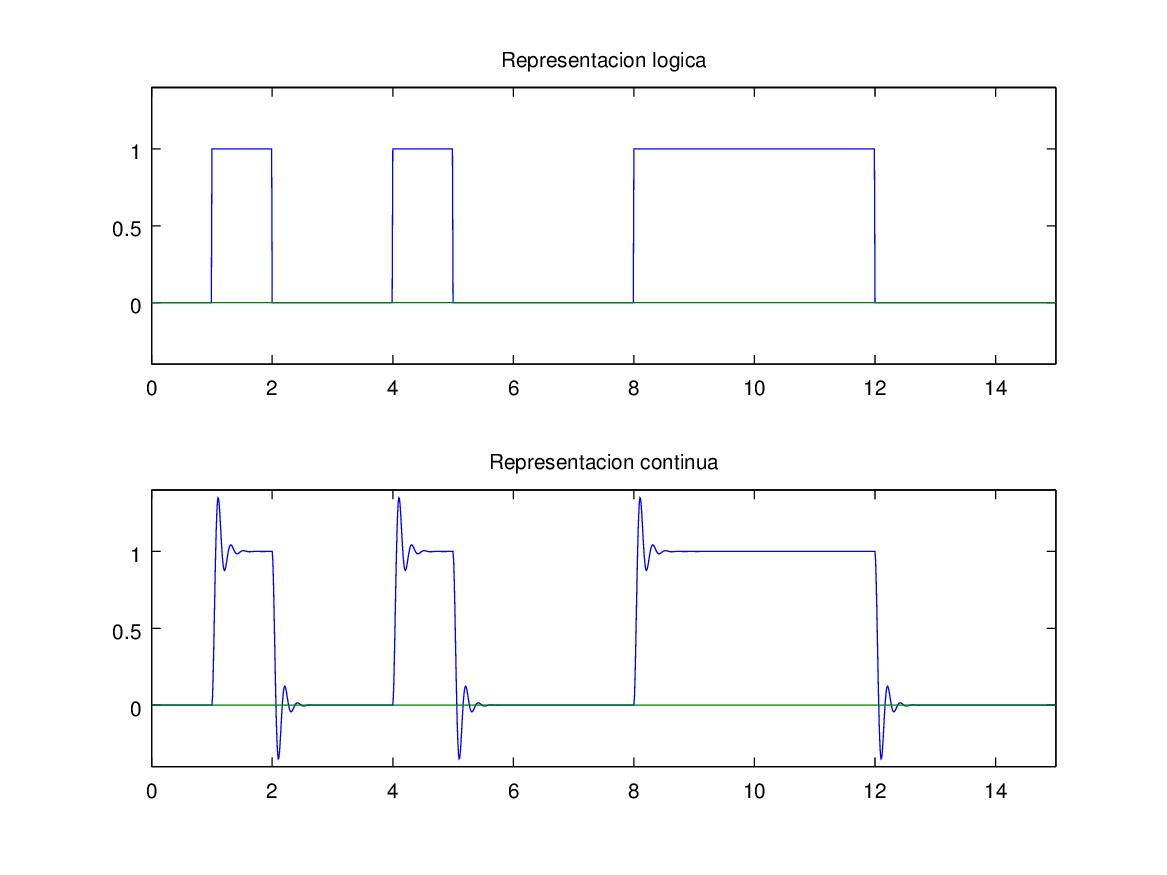
\includegraphics[height=3in]{./graphics/diversa.eps}
    \caption{Diversas representaciones de la misma se\~{n}al.}
    \label{diversaeps}
  \end{figure}

\item Consideremos ahora la funci\'{o}n de tiempo continuo
  \begin{equation}
    x\left(t\right) =\cos\left( 2 \, t\right), 
  \end{equation}
  Veamos su representaci\'{o}n en la Fig. (\ref{cos2tcoarseps}). Es
  evidente que en realidad tenemos secuencias de puntos, o sea
  se\~{n}ales de tiempo discreto, unidos por rectas de forma tal de
  dar la impresi\'{o}n de una se\~{n}al de de tiempo continuo cuando
  se la observa a una distancia adecuada.  Toda se\~{n}al procesada
  con una computadora es de tiempo discreto, porque las computadoras
  solo pueden procesar una cantidad finita y numerable de pedacitos de
  informaci\'{o}n (bits, en ingl\'{e}s). Lo que hacemos es graficar de
  forma tal que aceptamos lo que vemos como (un s\'{\i}mbolo de) una
  se\~{n}al de tiempo continuo.
  \begin{figure}
    \centering
    
\includegraphics[height=3in]{./py-graphics/target/cos2tcoarse.png}
    \caption{Es posible notar la discretizaci\'{o}n de esta
      funci\'{o}n ``continua''.}
    \label{cos2tcoarseps}
  \end{figure}
\end{enumerate}


%\subsection{Ejercicios para hacer}
%
%\begin{enumerate}
%\item En sus propias palabras, defina informaci\'{o}n, ruido, comunicaci\'{o}n, se\~{n}ales, sistemas, tiempo continuo, tiempo discreto, procesamiento, modelado, an\'{a}lisis, dise\~{n}o.
%
%\item De ejemplos de sistemas de tiempo continuo y discreto.
%
%\item \textquestiondown cual es la diferencia entre la informaci\'{o}n ``anal\'{o}gica'' (se\~{n}al de tiempo continuo) y la informaci\'{o}n ``digital'' (se\~{n}al de tiempo discreto)?
%\end{enumerate}

\section{Muestreo y cuantización}

El muestreo es la conversión de una señal de tiempo continuo $x(t)$ en una señal de tiempo discreto $x[n]$, tomando muestras de la señal en intervalos regulares de tiempo
\begin{equation}
	x[n] = x(n \, T_{s}).
\end{equation}
El muestreo se realiza para poder procesar la señal digitalmente, ya que la los sistemas digitales solo pueden trabajar con señales de tiempo discreto. El proceso de muestreo se realiza mediante un conversor analógico-digital (ADC), que toma muestras de la señal analógica a intervalos regulares $T_{s}$ (en el caso más común).

Además, los sistemas digitales necesitan que las señales esten cuantizadas.
La cuantización es la asignación de valores enteros a cada muestra y se realiza mediante un proceso de redondeo o truncamiento, que convierte los valores analógicos continuos (números reales) en valores discretos (números enteros en base 2). El nivel de cuantización se define por la cantidad de bits utilizados para representar cada muestra. Por ejemplo, una cuantización de $8$ bits produce $256$ posibles valores discretos para cada muestra.

Cabe aclarar que existen muestreos con intervalos $T_{s}$ variable o adaptivo.

\section{Propiedades de las se\~{n}ales}

\subsection{Se\~{n}ales acotadas y no acotadas de tiempo continuo}

Una se\~{n}al de tiempo continuo $x(t)$ es \textbf{acotada} si existe un n\'{u}mero real finito $M$ que
es mayor que el valor absoluto de $x(t)$ para todo valor de $t$
\begin{equation}
  |x(t)| < M,
\end{equation}

Una se\~{n}al de tiempo continuo $x(t)$ es \textbf{no acotada} si
existe $t_{1}$ tal que
\begin{equation}
  \begin{array}{c}
    Lim                     \\
    t \rightarrow t_{1}     
  \end{array}
  |x(t)| = \infty.
\end{equation}

\subsection{Se\~{n}ales acotadas y no acotadas de tiempo discreto}

Una se\~{n}al de tiempo discreto $x[n]$ es \textbf{acotada} si existe un n\'{u}mero real finito $M$ que
es mayor que el valor absoluto de $x[n]$ para todo valor de $n$
\begin{equation}
  |x[n]| < M,
\end{equation}.

Una se\~{n}al de tiempo discreto $x[n]$ es \textbf{no acotada} si
existe un tiempo $n_{1}$ tal que
\begin{equation}
  \begin{array}{c}
    Lim                     \\
    n \rightarrow n_{1}     
  \end{array}
  |x[n]| = \infty.
\end{equation}

\subsection{Se\~{n}ales infinitas y finitas, lateral derecha o lateral
  izquierda, causales y anticausales (tiempo continuo)}

Esto se refiere al momento en que las señales empiezan y terminan.

\begin{enumerate}
\item Una se\~{n}al $x(t)$ es finita si su valor es nulo antes de un
  tiempo de inicio $t_{1}$ y despu\'{e}s de un tiempo de
  finalizaci\'{o}n $t_{2}$. En caso contrario, la se\~{n}al es
  infinita.

\item Note que estas definiciones implican que para que una se\~{n}al
  sea infinita uno solo de ambos tiempos $t_{1}$ y $t_{2}$ necesita
  ser infinito mientras que el otro puede ser finito.
        
\item Una se\~{n}al $x(t)$ es infinita lateral derecho si $t_{2}
  \rightarrow \infty$ y $t_{1}$ tiene un valor finito.
        
\item Una se\~{n}al $x(t)$ es infinita lateral izquierdo si $t_{1}
  \rightarrow -\infty$ y $t_{2}$ tiene un valor finito.
        
\item Una se\~{n}al $x(t)$ es causal si es infinita lateral derecha y
  adem\'{a}s $t_{1} = 0$.
        
\item Una se\~{n}al $x(t)$ es nocausal si es infinita lateral
  izquierda y adem\'{a}s $t_{2} = 0$.

\item Note que una se\~{n}al puede ser infinita y acotada a la vez.
  Por ejemplo, $x(t) = cos(t)$.
\end{enumerate}

\subsection{Se\~{n}ales infinitas y finitas, lateral derecha o lateral
  izquierda, causales y anticausales (tiempo discreto)}

\begin{itemize}
\item Una se\~{n}al $x[n]$ es finita si su valor es nulo antes de un
  tiempo de inicio $n_{1}$ y despu\'{e}s de un tiempo de
  finalizaci\'{o}n $n_{2}$. En caso contrario, la se\~{n}al es
  infinita.

\item Note que estas definiciones implican que para que una se\~{n}al
  sea infinita uno solo de ambos tiempos $n_{1}$ y $n_{2}$ necesita
  ser infinito mientras que el otro puede ser finito.
        
\item Una se\~{n}al $x[n]$ es infinita lateral derecho si $n_{2}
  \rightarrow \infty$ y $n_{1}$ tiene un valor finito.
        
\item Una se\~{n}al $x[n]$ es infinita lateral izquierdo si $n_{1}
  \rightarrow -\infty$ y $n_{2}$ tiene un valor finito.
        
\item Una se\~{n}al $x[n]$ es causal si es infinita lateral derecha y
  adem\'{a}s $n_{1} = 0$.
        
\item Una se\~{n}al $x[n]$ es nocausal si es infinita lateral
  izquierda y adem\'{a}s $n_{2} = 0$.

\item Note que una se\~{n}al puede ser infinita y acotada a la vez.
  Por ejemplo, $x[n] = cos[n]$.
\end{itemize}

\subsection{Se\~{n}ales pares de tiempo continuo}

Una se\~{n}al de tiempo continuo es par si verifica la condici\'{o}n
\begin{equation}
  x(-t)=x(t).
\end{equation}

\subsubsection{Ejemplo}

Considere la siguiente ecuaci\'{o}n
\begin{equation}
  \cos (-t)=\cos (t).
\end{equation}
Vea la Fig. (\ref{contpareps}). Existe simetr\'{\i}a vertical, o
respecto al eje de absisas.

\begin{figure}
  \centering
  
\includegraphics[height=3in]{./py-graphics/target/contpar.png}
  \caption{Funci\'{o}n par (tiempo continuo)}
  \label{contpareps}
\end{figure}

\subsection{Se\~{n}ales pares de tiempo discreto}

Una se\~{n}al de tiempo discreto es par si verifica la condici\'{o}n
\begin{equation}
  x[-n]=x[n].
\end{equation}

\subsubsection{Ejemplo}

Considere la siguiente funci\'{o}n
\begin{equation}
  x[-n]=\frac{(-n)^{2}}{10}=\frac{n^{2}}{10}=x[n].
\end{equation}
Vea la Fig. (\ref{discpareps}). La gr\'{a}fica es invariante para una
rotaci\'{o}n de $\pi$ radianes.

\begin{figure}
  \centering
  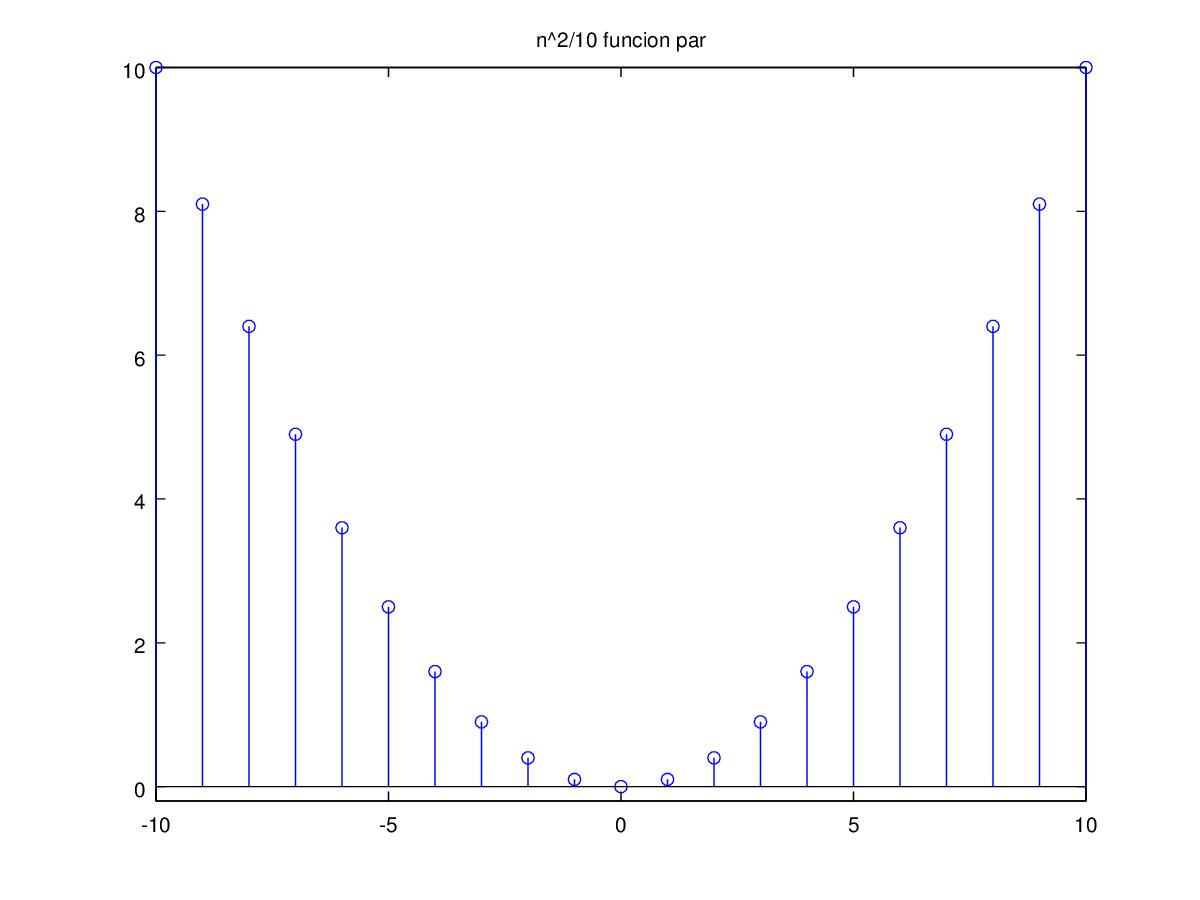
\includegraphics[height=3in]{./graphics/discpar.eps}
  \caption{Funci\'{o}n par (tiempo discreto). La gr\'{a}fica es
    invariante para una rotaci\'{o}n de $\pi$ radianes.}
  \label{discpareps}
\end{figure}

\subsection{Se\~{n}ales impares de tiempo continuo}

Una se\~{n}al de tiempo discreto es impar si verifica la condici\'{o}n
\begin{equation}
  x(-t)=-x(t).
\end{equation}

\subsubsection{Ejemplo}

Considere la siguiente funci\'{o}n
\begin{equation}
  \sin (-t)=-\sin (t).
\end{equation}
Vea la Fig. (\ref{contimpareps})

\begin{figure}
  \centering
  
\includegraphics[height=3in]{./py-graphics/target/contimpar.png}
  \caption{Funci\'{o}n impar (tiempo continuo)}
  \label{contimpareps}
\end{figure}

\subsection{Se\~{n}ales impares de tiempo discreto}

Una se\~{n}al de tiempo continuo es impar si verifica la condici\'{o}n
\begin{equation}
  x[-n]=-x[n].
\end{equation}

\subsubsection{Ejemplo}

Considere la siguiente funci\'{o}n
\begin{equation}
  x[-n]=\left( -n\right) ^{3}=-n^{3}=-x[n].
\end{equation}
Vea la Fig. (\ref{discimpareps}).

\begin{figure}
  \centering
  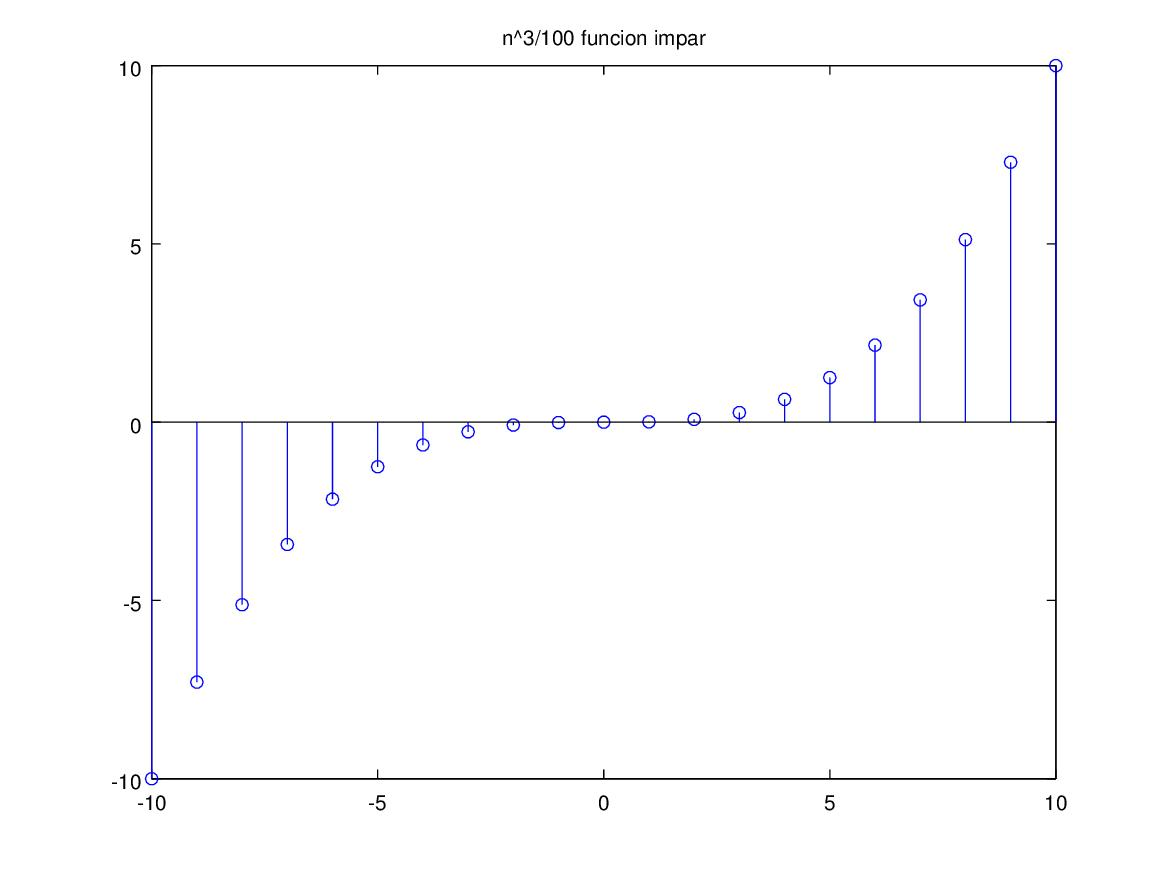
\includegraphics[height=3in]{./graphics/discimpar.eps}
  \caption{Funci\'{o}n impar (tiempo discreto)}
  \label{discimpareps}
\end{figure}

\subsection{Componentes par e impar de una se\~{n}al de tiempo
  continuo}

Una se\~{n}al de tiempo continuo puede descomponerse en componentes
par e impar
\begin{equation}
  x(t) = par(x(t)) + impar(x(t)),
\end{equation}
definiendo
\begin{eqnarray}
  par\left( x\left( t\right) \right) &=&\frac{1}{2}\left( x\left( t\right)
    +x\left( -t\right) \right) , \\
  impar\left( x\left( t\right) \right) &=&\frac{1}{2}\left( x\left( t\right)
    -x\left( -t\right) \right) .
\end{eqnarray}

\subsubsection{Ejemplo}

Vea la Fig. (\ref{contparimpareps}).

\begin{figure}
  \centering
  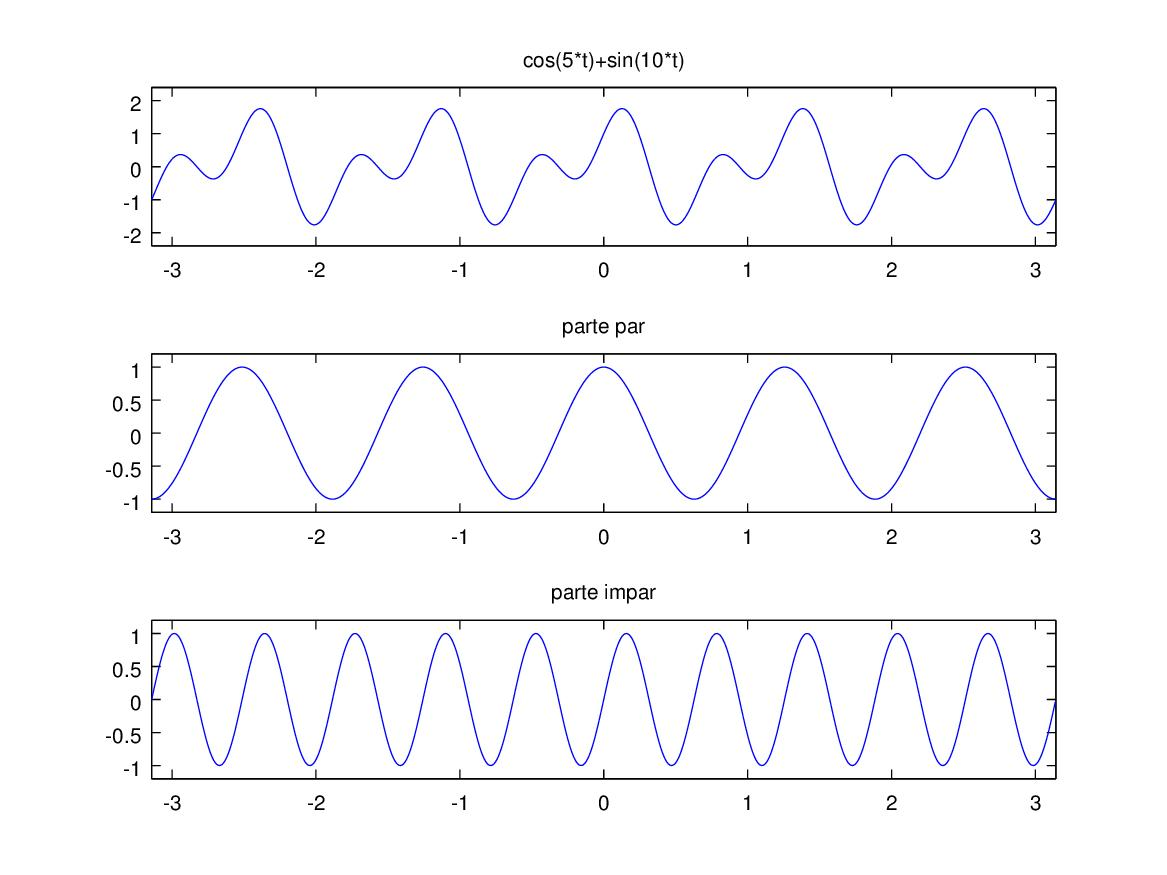
\includegraphics[height=3in]{./graphics/contparimpar.eps}
  \caption{Primer gr\'{a}fico: una funci\'{o}n con componentes pares e impares (tiempo continuo). Segundo gr\'{a}fico: componente par. Tercer gr\'{a}fico: componente impar. 
}
  \label{contparimpareps}
\end{figure}

\subsection{Componentes par e impar de una se\~{n}al de tiempo discreto}

Una se\~{n}al de tiempo discreto puede descomponerse en componentes
par e impar
\begin{equation}
  x[n] = par(x[n]) + impar(x[n]),
\end{equation}
definiendo
\begin{eqnarray}
  par\left( x\left[ n\right] \right) &=&
  \frac{1}{2}\left( x\left[ n\right] +x\left[ -n\right] \right) , \\
  impar\left( x\left[ n\right] \right) &=&
  \frac{1}{2}\left( x\left[ n\right] -x\left[ -n\right] \right) .
\end{eqnarray}

\subsubsection{Ejemplo}
Vea la Fig. (\ref{discparimpareps}).

\begin{figure}
  \centering
  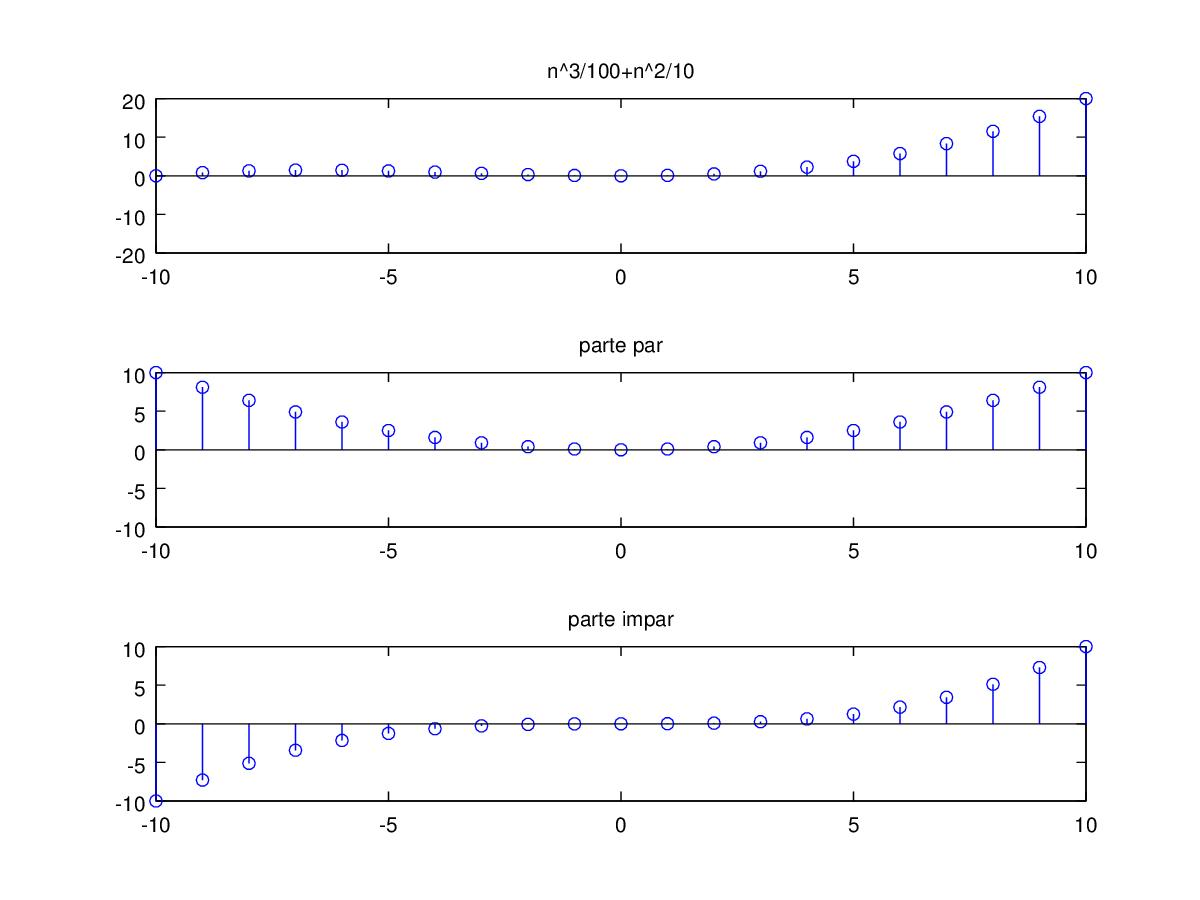
\includegraphics[height=3in]{./graphics/discparimpar.eps}
  \caption{Primer gr\'{a}fico: una funci\'{o}n con componentes pares e impares (tiempo discreto). Segundo gr\'{a}fico: componente par. Tercer gr\'{a}fico: componente impar.} 
  \label{discparimpareps}
\end{figure}

% \subsection{Ejercicios para hacer}
% Para cada uno de los tipos de se\~{n}ales considerados en esta secci\'{o}n de una definici\'{o}n y dos ejemplos con gr\'{a}ficos realizados en Matlab.

\section{Se\~{n}ales peri\'{o}dicas}

\subsection{Definici\'{o}n de per\'{\i}odo (tiempo continuo)}

Una se\~{n}al de tiempo continuo es peri\'{o}dica si existe un
n\'{u}mero $T$ denominado per\'{\i}odo tal que
\begin{equation}
  x(t)=x\left( t+ k \, T\right),
\end{equation}
donde $k$ es un número entero.

\subsection{Definici\'{o}n de per\'{\i}odo (tiempo discreto)}

Una se\~{n}al de tiempo discreto es peri\'{o}dica si existe un
n\'{u}mero $N$ denominado per\'{\i}odo tal que
\begin{equation}
  x[n]=x[n+ k \, N],
\end{equation}
donde $k$ es un número entero.

\subsection{Ejemplos}

\begin{enumerate}
\item Vea la Fig. (\ref{perconteps}). El per\'{\i}odo es $T = 10$.

\item Vea la Fig. (\ref{perdisceps}). El per\'{\i}odo es $N = 10$.

\item Vea la Fig. (\ref{noperdisceps}). No existe un n\'{u}mero $N$ tal que
\begin{equation}
  x[n]=x[n+N].
\end{equation}
Esta se\~{n}al nos parece peri\'{o}dica porque puede dibujarse sobre
una se\~{n}al peri\'{o}dica de tiempo continuo, denominada envolvente.
\end{enumerate}

\begin{figure}
  \centering
  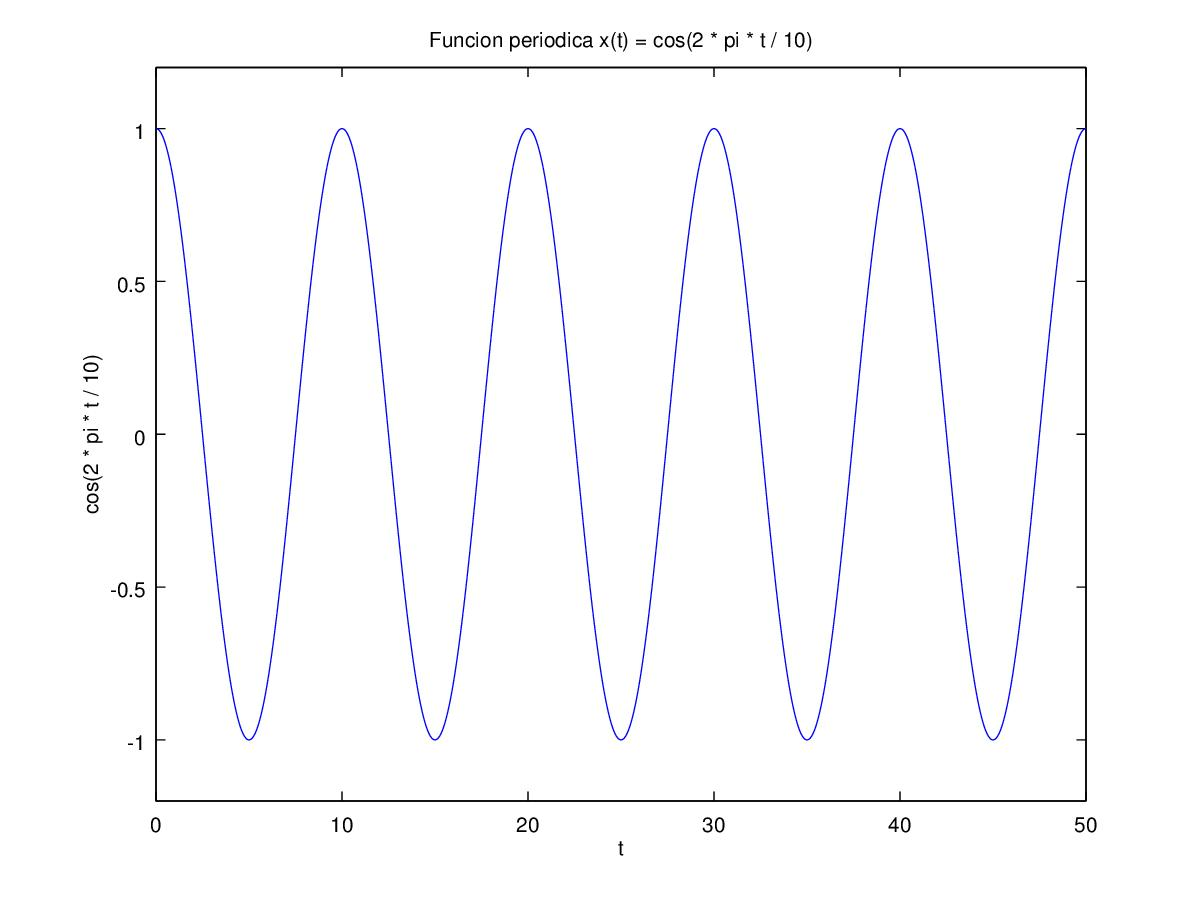
\includegraphics[height=3in]{./graphics/percont.eps}
  \caption{Se\~{n}al peri\'{o}dica de tiempo continuo $T = 10$}
  \label{perconteps}
  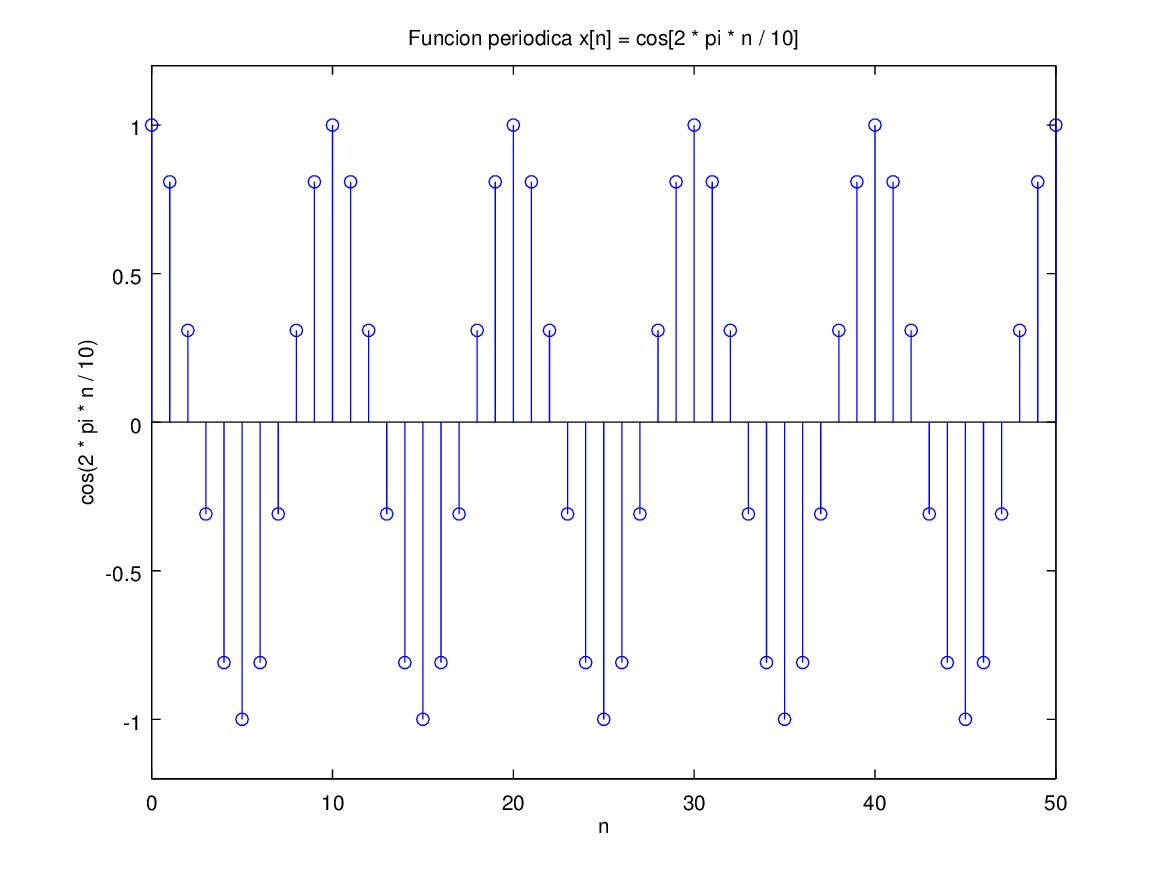
\includegraphics[height=3in]{./graphics/perdisc.eps}
  \caption{Se\~{n}al peri\'{o}dica de tiempo discreto $N = 10$}
  \label{perdisceps}
\end{figure}

\begin{figure}
  \centering
  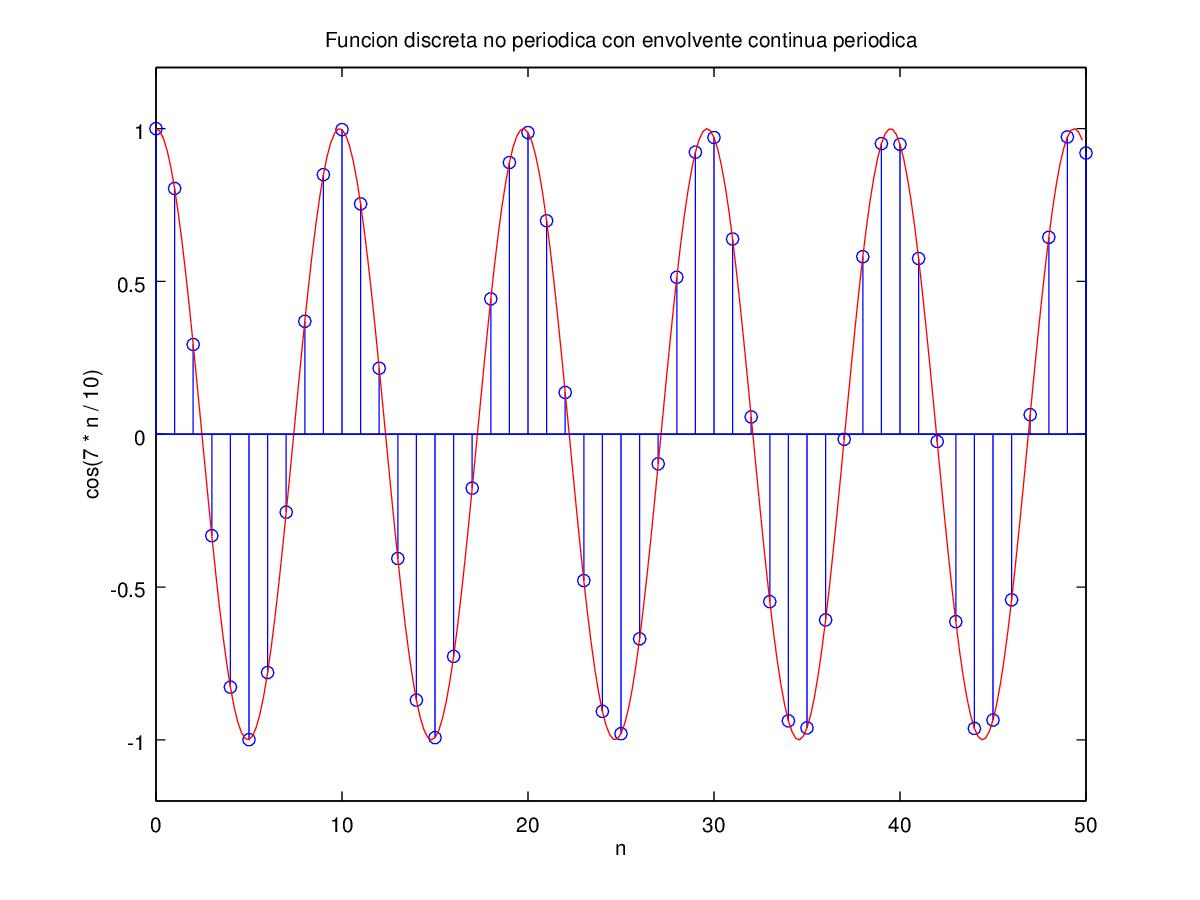
\includegraphics[height=3in]{./graphics/noperdisc.eps}
  \caption{Se\~{n}al de tiempo discreto que \textbf{NO} es
    peri\'{o}dica y que tiene una envolvente continua que si es
    peri\'{o}dica}
  \label{noperdisceps}  
\end{figure}

\subsection{Como encontrar los períodos de señales periódicas de tiempo continuo}

Las señales periódicas de tiempo continuo $x_{c}(t) = cos(\omega_{0} \, t)$ y
$x_{s}(t) = sin(\omega_{0} \, t)$ verifican la igualdad
\begin{equation}
 \omega_{0} \, T = 2 \, \pi.
\end{equation}
Por lo tanto $T = \frac{2 \, \pi}{\omega_{0}}$. 

\subsubsection{Ejemplos}

\begin{enumerate}
\item  $x\left( t\right) = 4 \, \cos \left( 5 \, \pi \, t\right),$ donde $\omega_{0} = 5 \, \pi$.
Podemos calcular el período
\begin{equation}
    5 \, \pi \, T= 2 \, \pi , \qquad T=\frac{2}{5}, \qquad \cos \left( 5 \, \pi \, \frac{2}{5}\right) = 
    \cos \left( 2 \, \pi \right) = \cos \left( 0\right) .
\end{equation}

\item  $x\left( t\right) =4\cos \left( 4 \, \pi \, t-\frac{\pi }{4}\right).$ Podemos calcular el período
\begin{equation}
    4 \, \pi \, T= 2 \, \pi , \qquad T=\frac{1}{2}, \qquad \cos \left( 4\pi \frac{1}{2} - \frac{\pi}{4}\right) = 
    \cos \left( 2 \, \pi - \frac{\pi}{4}\right) = \cos \left( -\frac{\pi}{4}\right) .
\end{equation}

\item  $x\left( t\right) =u\left( t\right) +4 \, \cos \left( 5 \, \pi \, t\right),$ 
no es periódica, porque 
\begin{equation}
u\left(\frac{-2}{5}\right) - 4 \, \cos \left(-5 \, \pi \, \frac{2}{5}\right) \neq u\left(\frac{2}{5}\right) - 4 \, \cos \left(5 \, \pi \, \frac{2}{5}\right). 
\end{equation}


\item  $x\left( t\right) =u\left( t\right) -\frac{1}{2}.$ No es periódica.

\item  $x\left[ n\right] =4\cos \left( \pi \, n\right).$ En este caso veremos que debe cumplirse 
\begin{equation}
\pi \, N=2 \, \pi , N=2.
\end{equation}

\item  $x\left[ n\right] =4\sin \left( 3 \, n\right).$ En  este caso veremos que $3 \, N \neq 2 \, \pi$. Por lo tanto $x[n]$ no es periódica.

\item  $x\left[ n\right] =4\cos \left( \pi n-2\right),$ es periódica con $N = 2$.

\item  $x\left[ n\right] =\left( -1\right) ^{n}$ es periódica con $N = 2$.

\end{enumerate}

% \subsection{Ejercicios para hacer}
% 
% \textquestiondown Cu\'{a}l es la se\~{n}al peri\'{o}dica de tiempo discreto que var\'{\i}a m\'{a}s rapidamente? \textquestiondown y
% m\'{a}s lentamente?
% 
% Escriba y grafique al menos dos funciones peri\'{o}dicas de distinta frecuencia (tiempo discreto).

\section{Se\~{n}ales exponenciales}

\subsection{Repaso de n\'{u}meros complejos}

Vamos a considerar distintos conceptos en los cuales emplearemos
n\'{u}meros complejos.  Por lo tanto, nos conviene recordar ciertas
notaciones y operaciones.

\subsubsection{Unidad imaginaria}

Definimos la unidad imaginaria como
\begin{equation}
  j = \sqrt{-1}.
\end{equation}
Por lo tanto, cumple con la igualdad
\begin{equation}
  j^{2} = -1.
\end{equation}

\subsubsection{N\'{u}meros complejos}

El conjunto de los n\'{u}meros complejos se simboliza $C$ y sus
elementos se representan en forma cartesiana como $a + b \, j$,
donde $a \in R$, $b \in R$, y $j$ es la unidad imaginaria.

\subsubsection{N\'{u}meros complejos conjugados}

Llamamos n\'{u}meros complejos conjugados a un par de n\'{u}meros que
simbolizamos $z$ y $\overline{z}$
\begin{equation}
  \begin{array}{ll}
    z =             &       a + j b,                        \\
    & \\
    \overline{z}    =       &       \overline{a + j b} = a - j b,
  \end{array}
\end{equation}
donde $a \in R$, $b \in R$, y $j$ es la unidad imaginaria.

\subsubsection{Parte real de un n\'{u}mero complejo}

Definimos a la funci\'{o}n parte real de un n\'{u}mero complejo como
\begin{equation}
  \Re{ \left( a + j b \right)} = a.
\end{equation}
Es sencillo deducir la propiedad
\begin{equation}
  \Re{ \left( a + j b \right)} = 
  \frac{(a + j b) + \overline{(a + j b)}}{2} =  \frac{(a + j b) + (a - j b)}{2} = a.
\end{equation}

\subsubsection{Parte imaginaria de un n\'{u}mero complejo}

Definimos a la funci\'{o}n parte imaginaria de un n\'{u}mero complejo
como
\begin{equation}
  \Im{\left( a + j b \right)} = b.
\end{equation}
Es sencillo deducir la propiedad
\begin{equation}
  \Im{ \left( a + j b \right)} = 
  \frac{(a + j b) - \overline{(a + j b)}}{2 j} =  \frac{(a + j b) - (a - j b)}{2 j} = b.
\end{equation}

\subsubsection{M\'{o}dulo de un n\'{u}mero complejo}

Definimos a la funci\'{o}n m\'{o}dulo de un n\'{u}mero complejo como
\begin{equation}
  \| a + j b \| = \sqrt{\left(a + j b\right)\left(a - j b\right)} = \sqrt{ a^{2} + b^{2}}.
\end{equation}
Por su definici\'{o}n, es un n\'{u}mero real igual o mayor que $0$.

\subsubsection{Fase de un n\'{u}mero complejo}

Definimos a la funci\'{o}n fase de un n\'{u}mero complejo como
\begin{equation}
  \angle a + j b  = \arctan (\frac{b}{a}).
\end{equation}

\subsubsection{Exponencial compleja}

Definimos la funci\'{o}n exponencial compleja como
\begin{equation}
  e^{a + j \, b} = e^{a} \, e^{j \, b} = e^{a} \, \left( \cos (b) + j \, \sin (b) \right),
\end{equation}

\subsubsection{Relaci\'{o}n de Euler}

La relaci\'{o}n de Euler es la igualdad
\begin{equation}
  e^{j b} =  \cos \left( b \right) + j \, \sin\left( b \right), \label{expeuler}
\end{equation}
Por lo tanto podemos escribir
\begin{equation}
  \cos \left( b \right) = \frac{e^{j \, b}+e^{-j \, b}}{2}, \label{coseuler}
\end{equation}
y
\begin{equation}
  \sin \left( b \right) = \frac{e^{j \, b}-e^{-j \, b}}{2j}. \label{sineuler}
\end{equation}


\subsubsection{Representaci\'{o}n en forma polar}

Un n\'{u}mero complejo $a + j b$ puede representarse en forma polar
\begin{equation}
  a + j b = \| a + j b\| e^{ j \, \angle{ a + j \, b} }.
\end{equation}

\subsection{Se\~{n}ales exponenciales de tiempo continuo}

Las se\~{n}ales exponenciales de tiempo continuo son las que tienen la
forma
\begin{equation}
  x(t)=R \, e^{a \, t}.
\end{equation}

\subsubsection{Se\~{n}ales exponenciales reales de tiempo continuo}

Se dice que la se\~{n}al exponencial es real si $R\in \Re$ y $a\in \Re$.

Si $ a > 0,$ entonces la se\~{n}al exponencial crece a medida que $t$ crece.

Si $ a < 0,$ entonces la se\~{n}al exponencial decrece a medida que $t$ crece.

\subsubsection{Se\~{n}ales exponenciales imaginarias de tiempo continuo}

Si $a = j \omega_{0}$ donde $j=\sqrt{-1}$ puede aplicarse la
relaci\'{o}n de Euler
\begin{equation}
  x\left( t\right) = 
  R \, e^{j \, \omega_{0} \, t}= 
  R \, \left(\cos \left( \omega_{0} \, t\right) +j \, \sin\left( \omega_{0} \, t\right) \right).
\end{equation}

\subsubsection{Se\~{n}ales exponenciales complejas de tiempo continuo}

La exponencial es compleja si $R$ es un n\'{u}mero real y $a$ es un n\'{u}mero complejo
\begin{equation}
  R\in \Re,
\end{equation}
y
\begin{equation}
  a=\gamma+j \, \omega_{0}\in C.
\end{equation}
La exponencial compleja puede evaluarse con la relaci\'{o}n de Euler
\begin{equation}
  x(t)= R \, e^{\gamma \, t}e^{j \, \omega_{0} \, t} = 
  R \, e^{\gamma \, t}\left( \cos \left( \omega_{0} \, t\right) + j \, \sin \left( \omega_{0} \, t\right) \right) ,
\end{equation}
donde
\begin{itemize}
\item $j=\sqrt{-1}$ es la unidad imaginaria
\item $R \, e^{\gamma \, t}$ es la envolvente,
\item Per\'{\i}odo $T$ y frecuencia $\omega_{0} = \frac{2 \, \pi}{T}$.
\end{itemize}

\subsubsection{Se\~{n}ales exponenciales generalizadas de tiempo continuo}
La exponencial es generalizada si tanto $R$ como $a$ son n\'{u}meros complejos
\begin{eqnarray}
  R &=&\alpha \, e^{j \, \theta }, \\
  a &=&\gamma + j \, \omega_{0}.
\end{eqnarray}
Podemos escribir entonces aplicando la relaci\'{o}n de Euler
\begin{equation}
  x\left( t\right) = R \, e^{a \, t}=
  \alpha \, e^{j \, \theta } \, e^{(\gamma + j \, \omega_{0}) \, t} = 
  \alpha \, e^{j \, \theta } \, e^{\gamma \, t} \, e^{j \, \omega_{0} \, t},
\end{equation}
\begin{equation}
  x\left( t\right) = R \, e^{a \, t}=
  \alpha \, e^{j \, \theta } \, e^{(\gamma + j \, \omega_{0}) \, t} = 
  \alpha \, e^{\gamma \, t} \, e^{j \, (\omega_{0} \, t + \theta)},
\end{equation}
\begin{equation}
  x\left( t\right) = R \, e^{a \, t}=
  \alpha \, e^{\gamma t}
  \left( \cos \left( \omega_{0} \, t+\theta \right) +
    j \, \sin \left( \omega_{0} \, t+\theta \right) \right) ,
\end{equation}
donde
\begin{itemize}
\item $j=\sqrt{-1}$ es la unidad imaginaria,
\item $\alpha e^{\gamma t}$ es la envolvente,
\item $\theta$ es la fase,
\item $\omega_{0}$ la frecuencia.
\end{itemize}

\subsection{Propiedades de la se\~{n}al exponencial imaginaria de tiempo continuo}

\subsubsection{Per\'{\i}odo y frecuencia}

Consideremos una se\~{n}al peri\'{o}dica de tiempo continuo con período $T_{0}$
\begin{equation}
  x\left( t\right) = x\left( t+T_{0}\right) .
\end{equation}
Para verificar que una se\~{n}al exponencial imaginaria de tiempo continuo sea
peri\'{o}dica podemos factorear
\begin{equation}
  R \, e^{j \, \omega_{0} \, t}= 
  R \, e^{j \, \omega_{0} \, \left(t+T_{0}\right)}= 
  R \, e^{j \, \omega_{0} \, t} \, e^{j \, \omega_{0} \, T_{0}},
\end{equation}
Aplicando la relación de Euler, verificamos
\begin{equation}
  e^{j \, \omega_{0} \, T_{0}}=
  \cos \left( \omega_{0} \, T_{0}\right) +
  j \, \sin \left(\omega_{0} \, T_{0}\right) = cos(2 \, \pi) + j \, sin(2 \, \pi) = 1,
\end{equation}
y
\begin{equation} 
  T_{0} = \frac{2 \, \pi }{\left|\omega_{0}\right| }.
\end{equation}
La conclusi\'{o}n es que la se\~{n}al exponencial imaginaria de tiempo
continuo \textbf{siempre} es peri\'{o}dica porque siempre podemos
encontrar $T_{0}$ dado $\omega_{0}$.

\subsubsection{Funciones arm\'{o}nicas de tiempo continuo} 

Dada una se\~{n}al peri\'{o}dica
\begin{equation}
  x(t) = x(t + T),
\end{equation}
existen infinitas se\~{n}ales peri\'{o}dicas arm\'{o}nicas de frecuencia $\omega_{k} = k \, \omega_{0} = k \, \frac{2 \, \pi}{T}$,
y período $T_{k} = \frac{T_{0}}{k}$, para $k \in N$, $k > 0$.


\subsection{Se\~{n}ales exponenciales de tiempo discreto}

Consideremos ahora la se\~{n}al exponencial de tiempo discreto
\begin{equation}
  x\left[ n\right] = R \, e^{\beta \, n} = R \, \alpha^{n},
\end{equation}
donde definimos
\begin{equation}
  \alpha = e^{\beta}.
\end{equation}

\subsubsection{Se\~{n}ales exponenciales reales de tiempo discreto}

\begin{enumerate}
\item Decimos que la exponencial es real si 
$\alpha \in \Re$ y $\beta \in \Re$.

\item Si $\left| \alpha \right| >1,$ o sea $\beta >0,$ entonces la
  exponencial crece a medida que $n$ crece.

\item Si $\left| \alpha \right| <1,$ o sea $\beta <0,$ entonces la
  exponencial decrece a medida que $n$ crece.
\end{enumerate}

\subsubsection{Se\~{n}ales exponenciales imaginarias de tiempo discreto}

Si $\beta $ es un n\'{u}mero imaginario puro entonces 
$\alpha = e^{j \, \omega_{0}} \rightarrow \left| \alpha \right| =1,$ y por la relaci\'{o}n de Euler
\begin{equation}
  x\left[ n\right] = 
  e^{j \, \omega_{0} \, n}=
  \cos \left( \omega_{0} \, n\right) +j \, \sin\left( \omega_{0} \, n\right).
\end{equation}

\subsubsection{Se\~{n}ales exponenciales generalizadas de tiempo discreto}

Definimos a la se\~{n}al exponencial generalizada de tiempo discreto
como
\begin{equation}
  x\left[ n\right] = R \, \alpha^{n},
\end{equation}
donde
\begin{eqnarray}
  R &=&\left| R \, \right| e^{j\theta }, \\
  \alpha &=&\left| \alpha \right| \, e^{j \, \omega_{0}}.
\end{eqnarray}
Podemos escribir entonces
\begin{equation}
  x\left[ n\right] =R \, \alpha^{n}=
  \left| R \, \right| \left| \alpha \right|^{n} \, e^{j \, \theta } \, e^{j \, \omega_{0} \, n} = 
  \left| R \, \right| \left| \alpha \right|^{n} \, e^{j \, (\omega_{0} \, n + \theta)},
\end{equation}
y
\begin{equation}
  x\left[ n\right] =R \, \alpha^{n}=
  \left| R \, \right| \left| \alpha \right|^{n} \, 
  \left( \cos \left( \omega_{0} \, n+\theta \right) +j \, \sin\left(\omega_{0} \, n+\theta \right) \right) .
\end{equation}

\subsection{Propiedades de la se\~{n}al exponencial imaginaria de tiempo discreto}

\subsubsection{Per\'{\i}odo y frecuencia}

Supongamos una funci\'{o}n exponencial imaginaria de tiempo discreto que
tenga per\'{\i}odo $N$
\begin{equation}
 x[n] = x[n + N].
\end{equation}
Por lo tanto, debería ser
\begin{equation}
 e^{j \, \omega_{0} \, n} = e^{j \, \omega_{0} \, (n + N)}.
\end{equation}
Esto significa que $\omega_{0}$ cumple con la relaci\'{o}n
\begin{equation}
  e^{j \, \omega_{0}\left( n+N\right) }=
  e^{j \, \omega_{0} \, n} \, e^{j \, \omega_{0} \, N}=e^{j \, \omega_{0} \, n}
  \Leftrightarrow e^{j \, \omega_{0} \, N}=1\Leftrightarrow\omega_{0} \, N=2 \, \pi M,
\end{equation}
donde $M$ es un n\'{u}mero entero. 
Por lo tanto, el per\'{\i}odo debe ser
\begin{equation}
  N =\frac{2 \, \pi }{\omega_{0}} \, M.
\end{equation}
Entonces si $\omega_{0} = P \, 2 \, \pi$, donde $P$ es un número racional,
\begin{equation}
  N =\frac{2 \, \pi }{P \, 2 \, \pi} \, M = \frac{M}{P},
\end{equation}
y
\begin{equation}
  P = \frac{M}{N}.
\end{equation}

\textbf{Para que una exponencial imaginaria de tiempo discreto sea
  peri\'{o}dica, su frecuencia debe ser una fracci\'{o}n propia de
  $\pi$.}

\subsubsection{Igualdad entre se\~{n}ales exponenciales con frecuencias $\omega_{0}$ y $\omega_{0}+2 \, \pi $}

Consideremos la funci\'{o}n $e^{j\left( \omega_{0}+2 \, \pi \right) n}$
que puede ser simplificada de la siguiente forma
\begin{equation}
  e^{j\left( \omega_{0}+2 \, \pi \right) \, n} = 
  e^{j \, \omega_{0} \, n} \, e^{j \, 2 \, \pi n} = 
  e^{j \, \omega_{0} \, n},
\end{equation}
porque
\begin{equation}
  e^{j2 \, \pi \, n}=
  \cos \left( 2 \, \pi \, n\right) +j \, \sin \left(2 \, \pi \, n\right) = 1+j \, 0, \forall n \in -2,-1,0,1,2,....
\end{equation}
Esto significa que dos funciones exponenciales complejas de tiempo discreto de frecuencias que difieran en $2 \, \pi $ son iguales.

\subsubsection{Señales armónicas de tiempo discreto}

Dada una se\~{n}al peri\'{o}dica
\begin{equation}
  x[n] = x[n + N],
\end{equation}
existen a lo sumo $N$ se\~{n}ales peri\'{o}dicas arm\'{o}nicas de frecuencia $\omega_{k} = k \, \frac{2 \, \pi}{N}$ 
enumerables $0 \leq k < N$, porque sino fuera así, $\omega_{k + N} = \omega_{k} + 2 \, \pi$.

Por ejemplo, consideremos
\begin{equation}
	x[n]_{k} = e^{j \, k \, \frac{2 \, \pi \, M}{N}}.
\end{equation}
Supongamos ahora que $k = N + 1$. Entonces
\begin{equation}
	x[n]_{N+1} = e^{j \, (N + 1) \, \frac{2 \, \pi \, M}{N}} = e^{j \, N \, \frac{2 \, \pi \, M}{N}} \, e^{j \, \frac{2 \, \pi \, M}{N}} = 
	e^{j \, \frac{2 \, \pi \, M}{N}} = x[n]_{1},
\end{equation}
porque $e^{j \, N \, \frac{2 \, \pi \, M}{N}} = e^{j \, 2 \, \pi \, M} = 1.$

\subsection{La se\~{n}al exponencial imaginaria es el bloque constructivo de otras se\~{n}ales peri\'{o}dicas}

\begin{enumerate}
\item Para construir otras se\~{n}ales peri\'{o}dicas usaremos
  conjuntos de exponenciales imaginarias (o sea, varias se\~{n}ales exponenciales imaginarias) a las que simbolizaremos
  \begin{equation}
    \phi _{k}\left( t\right) .
  \end{equation}
        
\item Usaremos exponenciales complejas $\phi_{k}(t)$ arm\'{o}nicas con un per\'{\i}odo com\'{u}n $T_{0}$.
  
\item
  Definiendo la frecuencia fundamental
  \begin{equation}
    \omega_{0}=\frac{2 \, \pi }{T_{0}},
  \end{equation}
  podemos definir el conjunto de funciones arm\'{o}nicas
  \begin{equation}
    \phi _{k}\left( t\right) = e^{j \, k \, \omega_{0} \, t}, k=0,\pm 1,\pm 2,....
  \end{equation}
        
\item Con la definici\'{o}n de funci\'{o}n arm\'{o}nica dada en el
  punto $2$ podemos construir funciones peri\'{o}dicas escritas como
  sumatorias de exponenciales imaginarias (multiplicadas por coeficientes adecuados).

\item Para obtener funciones peri\'{o}dicas escritas como combinaciones lineales
  de funciones trigonom\'{e}tricas podemos usar las relaciones
  \begin{equation}
    \cos \left(a \, t \right) = \frac{e^{j \, a \, t} + e^{-j \, a \, t}}{2},
  \end{equation}
  y
  \begin{equation}
    \sin \left(a t \right) = \frac{e^{j \, a \, t} - e^{-j \, a \, t}}{2 \, j}.
  \end{equation}

\end{enumerate}

\subsubsection{Ejemplo}

Consideremos la se\~{n}al
\begin{equation}
  x(t)= e^{j2t} + e^{-j2t} + j e^{j3t} - j e^{-j3t},      \label{ejeperiodicauno}
\end{equation}
equivalente a
\begin{equation}
  x(t)= 2 \, \frac{e^{j \, 2 \, t} + e^{-j \, 2 \, t}}{2} + (2 \, j) \, j \, \frac{(e^{j \, 3 \, t} - e^{-j \, 3 \, t})}{2 \, j},
\end{equation}
y finalmente a
\begin{equation}
  x(t)= 2 \, \cos \left(2 \, t \right) - 2 \, \sin \left(3 \, t \right). \label{ejeperiodicados}
\end{equation}
Observe que como los sumandos de (\ref{ejeperiodicauno}) son complejos
conjugados, $x(t)$ resulta ser una funci\'{o}n real, como vemos en
(\ref{ejeperiodicados}).

\subsection{Comparaci\'{o}n de las se\~{n}ales peri\'{o}dicas de tiempo continuo y discreto}

\subsubsection{Se\~{n}al de tiempo continuo $e^{j \, \protect\omega_{0} \, t}$}

\begin{enumerate}
\item Distintas se\~{n}ales para distintos valores de $\omega_{0};$

\item Peri\'{o}dica para cualquier valor de $\omega_{0};$

\item Frecuencia fundamental $\omega_{0};$

\item Per\'{\i}odo fundamental $T = \frac{2 \, \pi}{\omega_{0}}.$
\end{enumerate}

\subsubsection{Se\~{n}al de tiempo discreto $e^{j \, \protect\omega_{0}n}$}

\begin{enumerate}
\item Id\'{e}nticas se\~{n}ales para $\omega_{0}$ y $\omega_{0}+2 \, \pi
  ;$

\item Peri\'{o}dica s\'{o}lo si $\omega_{0} \, N=2 \, \pi \, M,$ y $N$ y $M$ sin
  factores en com\'{u}n;

\item Frecuencia fundamental $\omega_{0};$

\item Per\'{\i}odo fundamental $N$ tal que $\frac{N}{M} = \frac{2 \, \pi }{\omega_{0}}.$
\end{enumerate}

% \subsection{Ejercicios para hacer}
% 
% Escriba ejemplos gr\'{a}ficos en Matlab de se\~{n}ales peri\'{o}dicas de tiempo continuo y discreto.

\section{Se\~{n}ales singulares}

A continuaci\'{o}n veremos unos objetos matem\'{a}ticos especiales que
nos permiten representar ciertas \textbf{se\~{n}ales singulares}, y
as\'{\i} desarrollar una teor\'{\i}a matem\'{a}tica \'{u}til.

\subsection{El impulso unitario (tiempo discreto)}

Se define el impulso unitario de tiempo discreto como
\begin{equation}
  \delta \left[ n\right] =\left\{ 
    \begin{array}{ll}
      0, & n\neq 0, \\ 
      1, & n=0.
    \end{array}
  \right.                \label{impunidiscdef}
\end{equation}
Vea la Fig. (\ref{impunidisceps}).

\begin{figure}
  \centering
  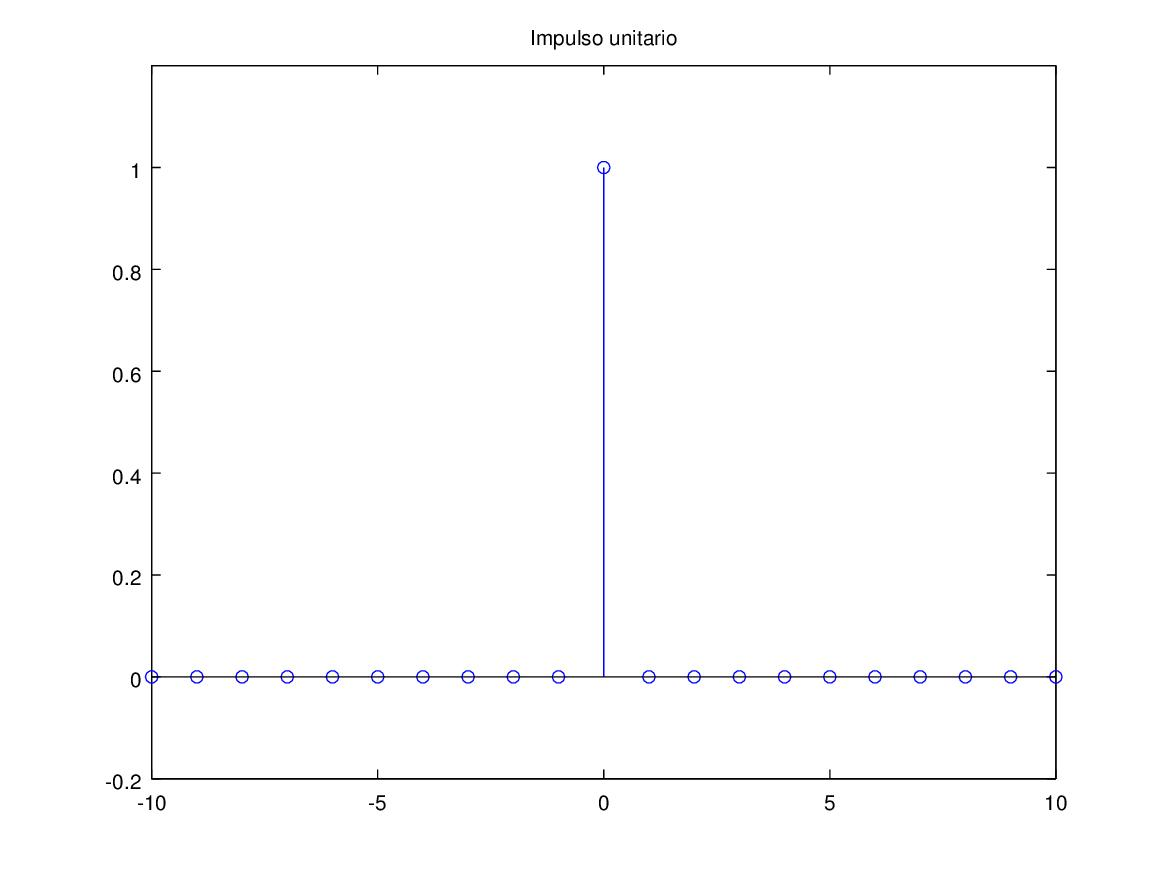
\includegraphics[height=3in]{./graphics/impunidisc.eps}
  \caption{Impulso unitario de tiempo discreto.}
  \label{impunidisceps}
\end{figure}

Podemos desplazar al impulso unitario en el tiempo. En este caso la
definici\'{o}n es
\begin{equation}
  \delta \left[ n - n_{0}\right] =\left\{ 
    \begin{array}{ll}
      0,      & n\neq n_{0}, \\ 
      1,      & n= n_{0}.
    \end{array}
  \right.
\end{equation}
Vea la Fig. (\ref{impunidiscdespeps}).

\begin{figure}
  \centering
  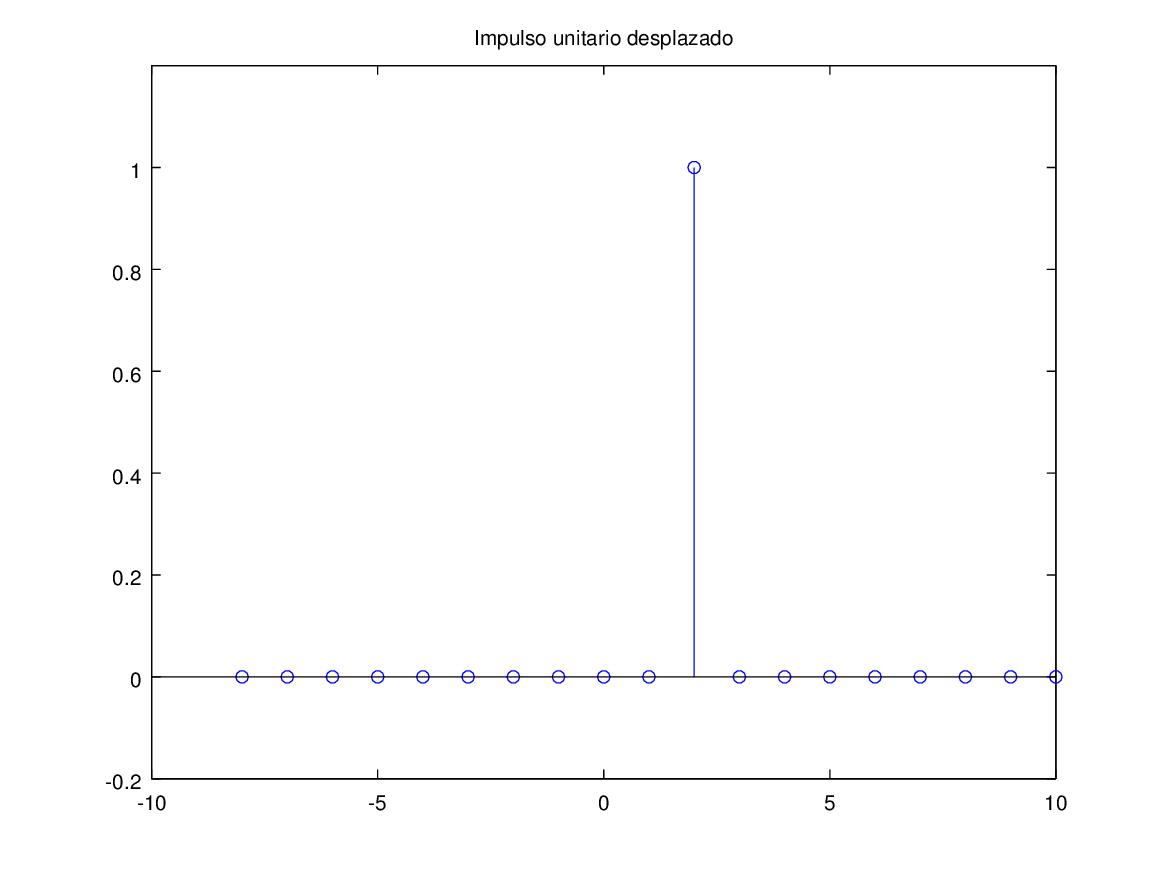
\includegraphics[height=3in]{./graphics/impunidiscdesp.eps}
  \caption{Impulso unitario de tiempo discreto desplazado.}
  \label{impunidiscdespeps}
\end{figure}

Tambi\'{e}n podemos multiplicar al impulso unitario por un valor real
$v$.  En este caso la definici\'{o}n es
\begin{equation}
  v \delta \left[ n - n_{0}\right] =\left\{ 
    \begin{array}{ll}
      0,      & n\neq n_{0}, \\ 
      v,      & n= n_{0}.
    \end{array}
  \right. 
\end{equation}
Vea la Fig. (\ref{impunidiscdespmulteps}).

\begin{figure}
  \centering
  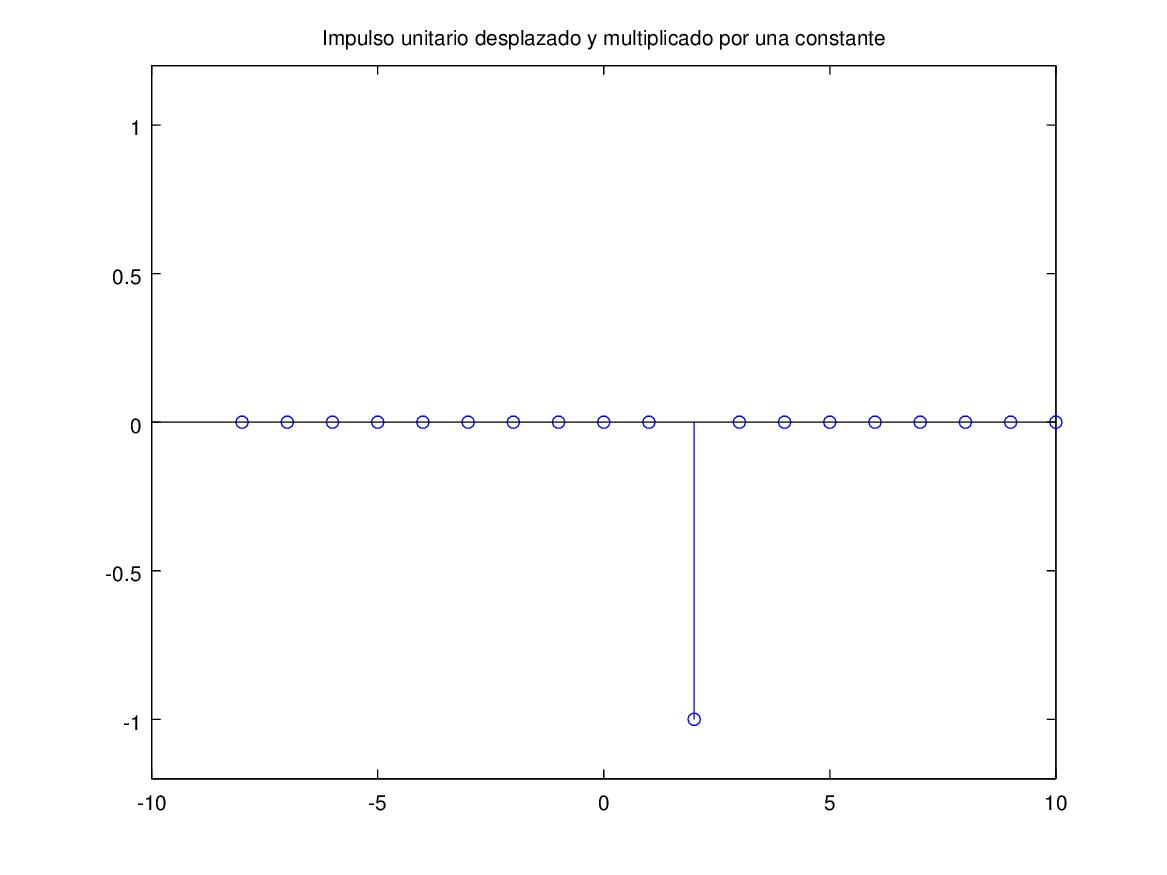
\includegraphics[height=3in]{./graphics/impunidiscdespmult.eps}
  \caption{Impulso unitario de tiempo discreto desplazado y
    multiplicado.}
  \label{impunidiscdespmulteps}
\end{figure}

\subsection{El escal\'{o}n unitario (tiempo discreto)}

Se define el escal\'{o}n unitario de tiempo discreto como
\begin{equation}
  u\left[ n\right] =\left\{ 
    \begin{array}{ll}
      0, & n<0, \\ 
      1, & n\geq 0.
    \end{array}
  \right.
\end{equation}
Vea la Fig. (\ref{escunidisceps}).

\begin{figure}
  \centering
  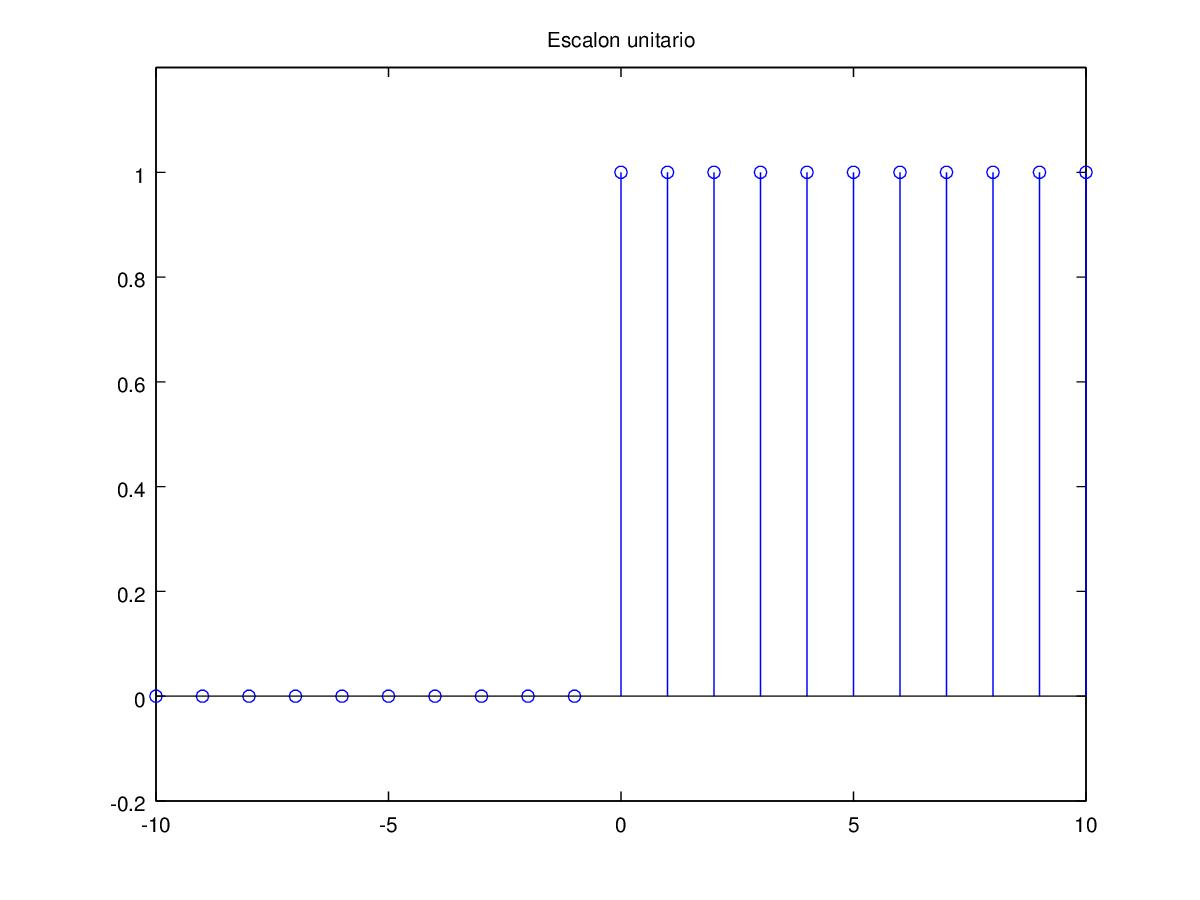
\includegraphics[height=3in]{./graphics/escunidisc.eps}
  \caption{Escal\'{o}n unitario de tiempo discreto.}
  \label{escunidisceps}
\end{figure}

Podemos desplazar al escal\'{o}n unitario en el tiempo. En este caso
la definici\'{o}n es
\begin{equation}
  u \left[ n - n_{0}\right] =\left\{ 
    \begin{array}{ll}
      0,      & n <    n_{0}, \\ 
      1,      & n \geq n_{0}.
    \end{array}
  \right.
\end{equation}
Vea la Fig. (\ref{escunidiscdespeps}).

\begin{figure}
  \centering
  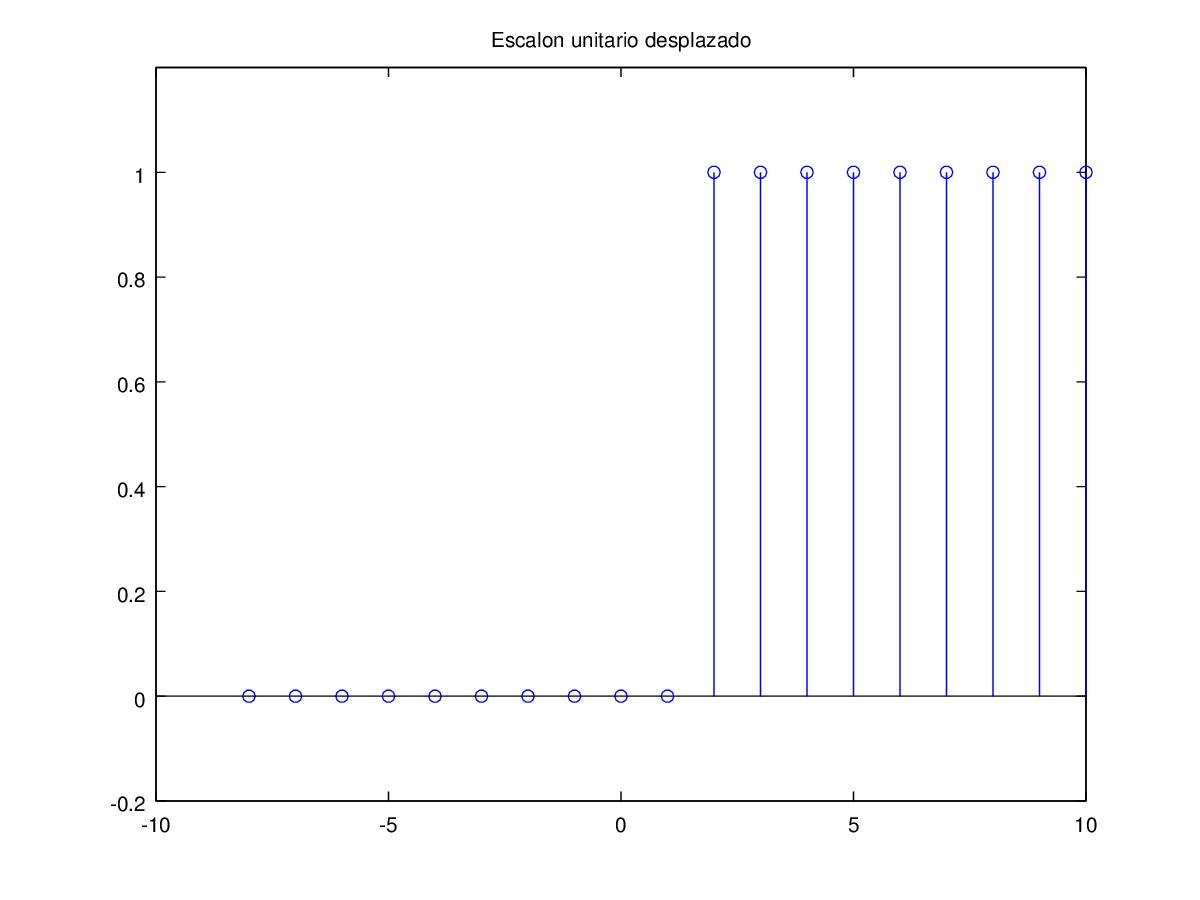
\includegraphics[height=3in]{./graphics/escunidiscdesp.eps}
  \caption{Escal\'{o}n unitario de tiempo discreto desplazado.}
  \label{escunidiscdespeps}
\end{figure}

Tambi\'{e}n podemos multiplicar al escal\'{o}n unitario por un valor
real $v$.  En este caso la definici\'{o}n es
\begin{equation}
  v u \left[ n - n_{0}\right] =\left\{ 
    \begin{array}{ll}
      0,      & n < n_{0}, \\ 
      v,      & n \geq n_{0}.
    \end{array}
  \right.
\end{equation}
Vea la Fig. (\ref{escunidiscdespmulteps}).

\begin{figure}
  \centering
  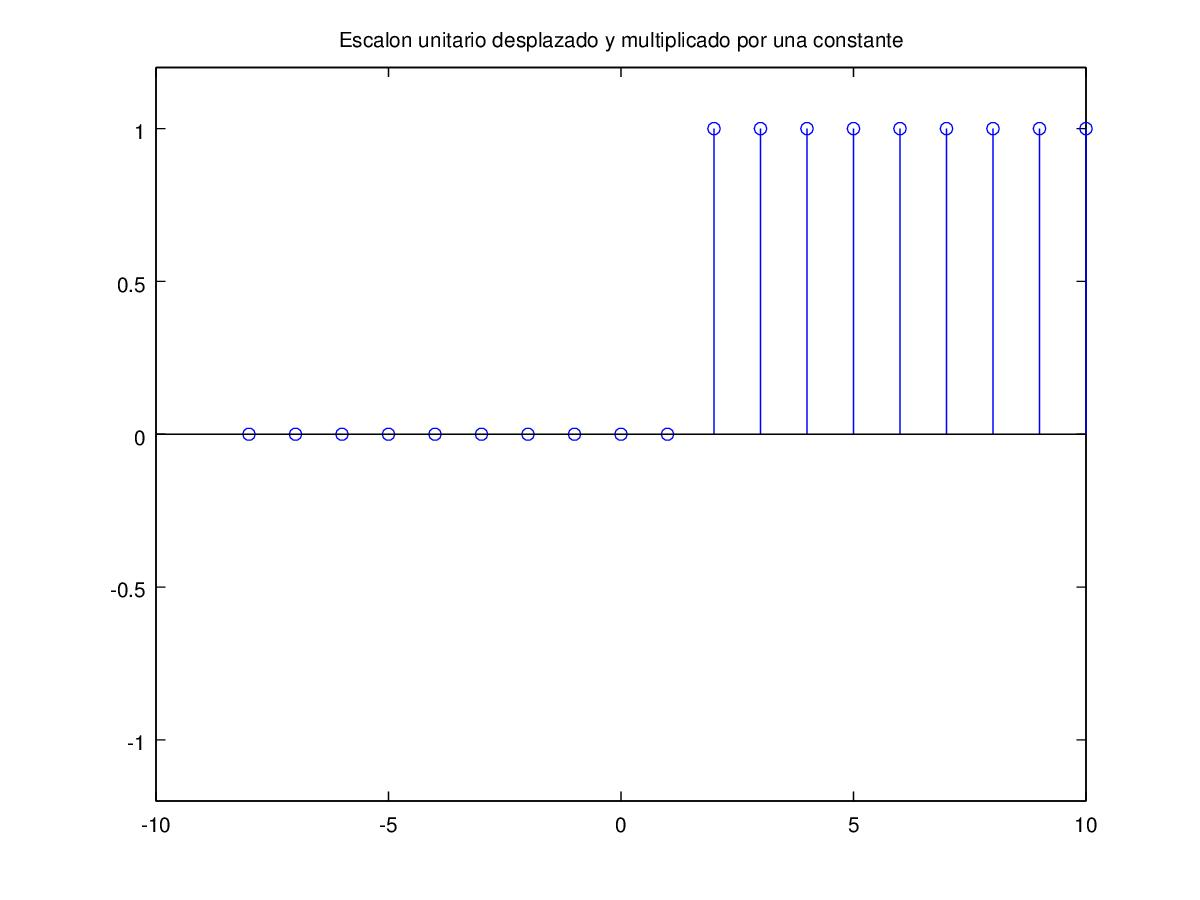
\includegraphics[height=3in]{./graphics/escunidiscdespmult.eps}
  \caption{Escal\'{o}n unitario de tiempo discreto desplazado y
    multiplicado.}
  \label{escunidiscdespmulteps}
\end{figure}

\subsection{Relaci\'{o}n entre impulso y escal\'{o}n (tiempo discreto)}

Las relaciones entre impulso y escal\'{o}n son las siguientes
\begin{eqnarray}
  \delta \left[ n\right] &=&u\left[ n\right] -u\left[ n-1\right] . \\
  u\left[ n\right] &=&\sum_{m=-\infty }^n\delta \left[ m\right] .
\end{eqnarray}
Cambiando $k=n-m$%
\begin{equation}
  u\left[ n\right] =\sum_{k=\infty }^{0}\delta \left[ n-k\right] ,
\end{equation}
o
\begin{equation}
  u\left[ n\right] =\sum_{k=0}^{\infty }\delta \left[ n-k\right] .
\end{equation}
Esta es la definici\'{o}n impl\'{i}cita del impulso, como la se\~{n}al
que sumada en el tiempo ``genera'' un escal\'{o}n. Vea la Fig.
(\ref{lecture02_text_gr10eps}).

Escribiendo
\begin{equation}
  u\left[ n\right] = 
\left(\sum_{k<n}^{\infty }\delta \left[n-k\right] \right) + 
\delta\left(0\right) + 
\left(\sum_{n<k}^{\infty }\delta \left[n-k\right] \right),
\end{equation}

\begin{figure}
  \centering
  \includegraphics[height=2in]{./graphics/lecture02_tex_gr10.eps}
  \caption{Impulso de tiempo discreto desplazado y
    multiplicado, y escalón unitario de tiempo discreto}
  \label{lecture02_text_gr10eps}
\end{figure}

\subsection{El escal\'{o}n unitario (tiempo continuo)}

Definimos el escal\'{o}n unitario de tiempo continuo como
\begin{equation}
  u\left( t\right) =\left\{ 
    \begin{array}{ll}
      0, & t < 0    \\ 
      1, & t > 0
    \end{array}
  \right.
\end{equation}
Observe que la funci\'{o}n tiene una discontinuidad en $t=0$.  Vea la
Fig. (\ref{lecture_text_gr9eps})


\subsection{El impulso unitario (tiempo continuo)}

Definimos el impulso unitario de tiempo continuo como
\begin{equation}
  u\left( t\right) =\int_{-\infty }^{t}\delta \left( \tau \right) d\tau . \label{escimpcont}
\end{equation}
Esta es la definici\'{o}n impl\'{i}cita del impulso, como la se\~{n}al
que integrada en el tiempo ``genera'' un escal\'{o}n.

\subsection{Construcci\'{o}n del impulso y el escal\'{o}n unitario}

La ecuaci\'{o}n (\ref{escimpcont}) nos da una definici\'{o}n de un
impulso pero no nos dice como construirlo. Para esto podemos ver al
impulso unitario como el l\'{\i}mite de una sucesi\'{o}n de funciones
de area unitaria.
\begin{enumerate}

\item Definamos una sucesi\'{o}n de funciones $r_{\Delta} \left( t -
    t_{0} \right) $ de \'{a}rea unitaria
  \begin{equation}
    r_{\Delta} \left( t - t_{0} \right) = \left \{
      \begin{array}{ll}
        0                       &       t < t_{0},                                              \\
        \frac{1}{\Delta}        &       t_{0}   \leq    t       \leq    t_{0} + \Delta,         \\
        0                       &       t_{0} + \Delta < t, 
      \end{array} 
    \right.
  \end{equation}
  donde $\Delta$ es una constante real no negativa. Vea la Fig.
  (\ref{sucimpconteps.1}). Esta no es la \'{u}nica forma de hacerlo, vea
  las Figs. (\ref{lecture02texgr7eps}) y (\ref{lecture02texgr8eps}).

\begin{figure}
  \centering
  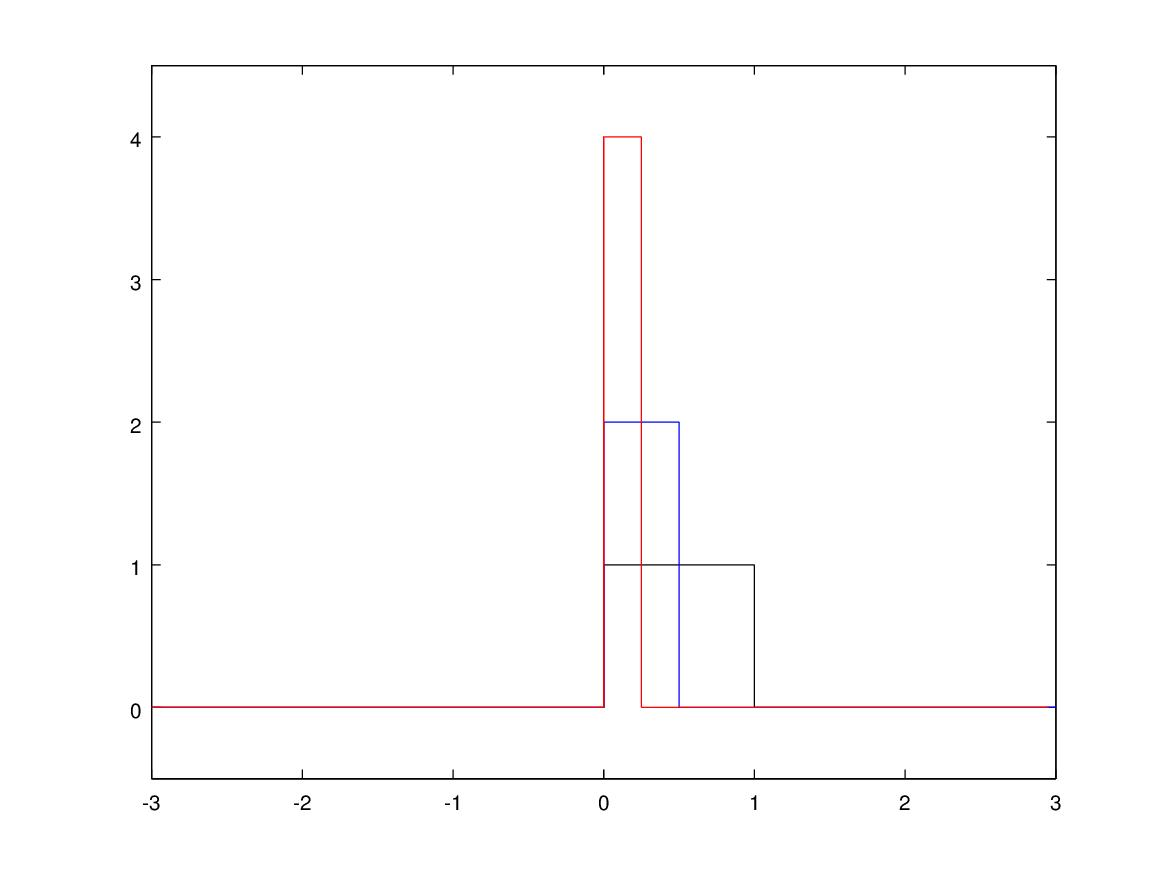
\includegraphics[height=3in]{./graphics/sucimpcont.eps}
  \caption{Sucesi\'{o}n de funciones que convergen a un impulso
    unitario de tiempo continuo.}
  \label{sucimpconteps.1}
\end{figure}

\begin{figure}
  \centering
  \includegraphics[height=3in]{./graphics/lecture02_tex_gr7.eps}
  \caption{Aproximaci\'{o}n del impulso unitario de tiempo continuo.}
  \label{lecture02texgr7eps}
\end{figure}

\begin{figure}
  \centering
  \includegraphics[height=3in]{./graphics/lecture02_tex_gr8.eps}
  \caption{Aproximaci\'{o}n del impulso unitario de tiempo continuo.}
  \label{lecture02texgr8eps}
\end{figure}

\item Tenemos entonces que el impulso $\delta \left( t \right)$ es el
  l\'{\i}mite
  \begin{equation}
    \delta \left( t - t_{0}\right) = 
    \begin{array}{l}
      Lim                             \\
      \Delta \rightarrow 0
    \end{array}
    r_{\Delta} \left( t - t_{0} \right).            \label{impunsuc}
  \end{equation}

\item Definamos tambi\'{e}n una sucesi\'{o}n de funciones $s_{\Delta}
  \left( t \right)$ dadas por
  \begin{equation}
    s_{\Delta} \left( t - t_{0} \right) = \left \{
      \begin{array}{ll}
        0,                      &       t < t_{0},                              \\
        \frac{t}{\Delta},       &       t_{0} \leq t \leq t_{0} + \Delta,       \\
        1,                      &       t_{0} + \Delta < t.
      \end{array}
    \right.         \label{escunsuc}
  \end{equation}
  Vea la Fig. (\ref{sucescconteps}).

\begin{figure}
  \centering
  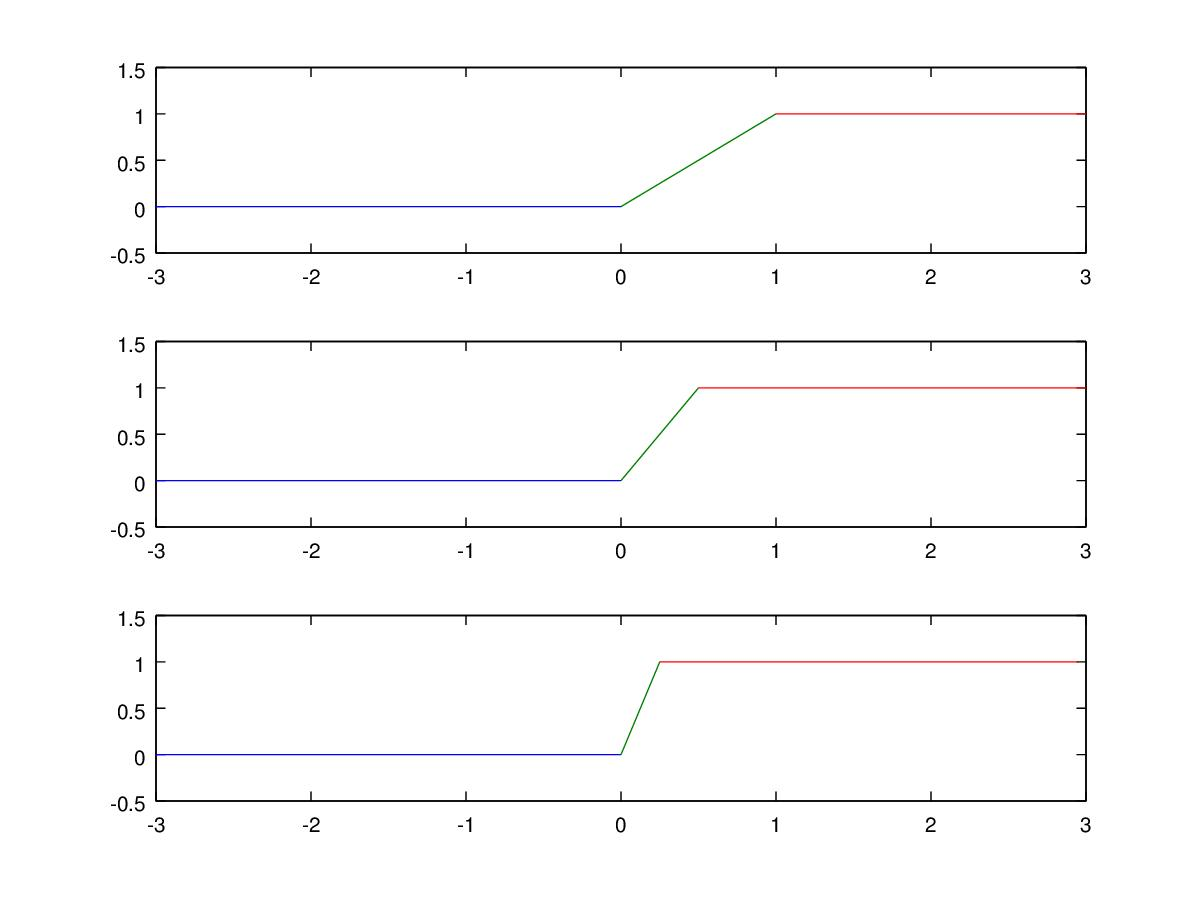
\includegraphics[height=3in]{./graphics/sucesccont.eps}
  \caption{Sucesi\'{o}n de funciones que convergen a un escal\'{o}n
    unitario de tiempo continuo.}
  \label{sucescconteps}
\end{figure}
        
\item Tenemos entonces que el escal\'{o}n $u \left( t \right)$ es el
  l\'{\i}mite
  \begin{equation}
    u \left( t - t_{0} \right) = 
    \begin{array}{l}
      Lim                             \\
      \Delta \rightarrow 0
    \end{array}
    s_{\Delta} \left( t - t_{0} \right).
  \end{equation}
  Vea la Fig. (\ref{lecture_text_gr9eps}).

  % \begin{figure}
  %   \centering
  %   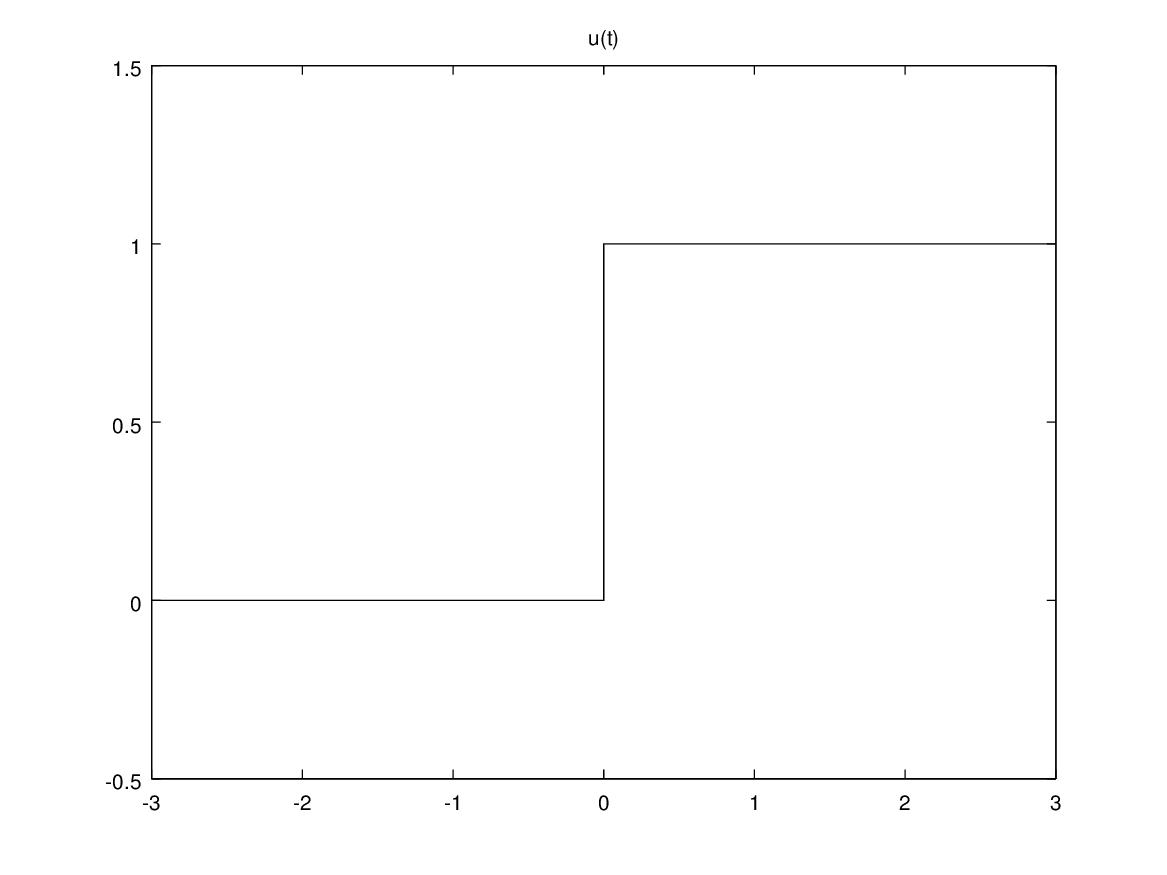
\includegraphics[height=3in]{./graphics/limesccont.eps}
  %   \caption{L\'{\i}mite de una sucesi\'{o}n de funciones que
  %     convergen a un escal\'{o}n unitario de tiempo continuo.}
  %   \label{limescconteps}
  % \end{figure}

\begin{figure}
  \centering
  \includegraphics[height=3in]{./graphics/lecture02_tex_gr9.eps}
  \caption{Escal\'{o}n unitario de tiempo continuo}
  \label{lecture_text_gr9eps}
\end{figure}
        
\end{enumerate}

\subsubsection{Impulso en el tiempo}

\begin{enumerate}
\item Un impulso de corriente en tiempo entrega una unidad de carga
  instan-t\'{a}neamente a un circuito.

\item Un impulso de fuerza en tiempo entrega un momento
  instant\'{a}neo a un mecanismo.
\end{enumerate}

\subsubsection{Impulso en el espacio}

\begin{enumerate}

\item Un impulso de masa en el espacio es una masa puntual.

\item Un impulso de densidad de carga en el espacio es una carga
  puntual.

\item Un impulso de intensidad de luz en el espacio es una luz
  puntual.
\end{enumerate}

% \subsection{Ejercicios para hacer}
% 
% Escriba las definiciones de las se\~{n}ales singulares expuestas en esta secci\'{o}n.
% 
% De ejemplos gr\'{a}ficos en Matlab.
% 
\section{Se\~{n}ales muestreadas}

El muestreo de se\~{n}ales es una operaci\'{o}n muy importante. Preste
atenci\'{o}n.  Veremos primero el muestreo en tiempo discreto, y despu\'{e}s en tiempo continuo.

\subsection{Tiempo discreto}

\begin{enumerate}
\item Recordemos la definici\'{o}n del impulso unitario de tiempo
  discreto
  \begin{equation}
    \delta \left[ n - n_{0}\right] =\left\{ 
      \begin{array}{ll}
        0, & n\neq n_{0}, \\ 
        1, & n = n_{0}.
      \end{array}
    \right.
  \end{equation}

\item Supongamos que tenemos una se\~{n}al $x[n]$. Podemos obtener una
  nueva se\~{n}al
  \begin{equation}
    z[n] = x[n] \delta[n - n_{0}],
  \end{equation}
  de la siguiente forma
  \begin{equation}
    z[n] = \left \{
      \begin{array}{ll}
        0       &       n \neq n_{0},   \\
        x[n_{0}]        & n  = n_{0}.
      \end{array}             \label{muesdiscre}
    \right.
  \end{equation}

\item Podemos resumir la operaci\'{o}n realizada en la ec.
  (\ref{muesdiscre}) como
  \begin{equation}
    x\left[ n\right] \delta \left[ n-n_{0}\right] =
    x\left[ n_{0}\right] \delta \left[ n-n_{0}\right], \label{claveuno}
  \end{equation}
  y la denominaremos muestreo en tiempo discreto.

\item La ec. (\ref{claveuno}) es una de las claves de esta materia.
  Por favor recuerdela.
\end{enumerate}

\subsection{Tiempo continuo}

\begin{enumerate}
\item Recordemos la definici\'{o}n \textbf{de la sucesi\'{o}n de
    funciones} cuyo l\'{\i}mite es el impulso unitario
  \begin{equation}
    r_{\Delta} \left( t - t_{0} \right) = \left \{
      \begin{array}{ll}
        0                       &       t < t_{0},                                              \\
        \frac{1}{\Delta}        &       t_{0} \leq      t       \leq    t_{0} + \Delta,         \\
        0                       &       t_{0} + \Delta < t ,
      \end{array} 
    \right.
  \end{equation}
  donde $\Delta$ es una constante real no negativa.

\item Supongamos que tenemos una se\~{n}al $x \left( t \right)$.
  Podemos obtener una nueva se\~{n}al
  \begin{equation}
    z \left( t \right) = x \left( t \right) \delta \left( t - t_{0}\right),
  \end{equation}
  de la siguiente forma
  \begin{enumerate}
  \item Construyamos una sucesi\'{o}n de funciones
    \begin{equation}
      z_{\Delta} \left( t \right) = \left \{
        \begin{array}{ll}
          0                                       &       t < t_{0},                              \\
          x\left( t_{0} \right) \frac{1}{\Delta}      &       t_{0} \leq t \leq t_{0} + \Delta,       \\
          0                                       &       t_{0} + \Delta < t,
        \end{array} 
      \right.
    \end{equation}
                        
  \item La funci\'{o}n $z \left( t \right)$ es el l\'{\i}mite de la
    sucesi\'{o}n cuando $\Delta \rightarrow 0$.
                        
  \end{enumerate}
  \begin{equation}
    z \left( t \right) = 
    x\left( t\right) \delta \left( t-t_{0}\right) =
    x\left( t_{0}\right) \delta \left(
      t-t_{0}\right) . \label{clavedos}
  \end{equation}

\item La ec. (\ref{clavedos}) es una de las claves de esta materia.
  Por favor recuerdela.
\end{enumerate}

% \subsection{Ejercicios para hacer}

% Escriba su propia versi\'{o}n de esta secci\'{o}n, con ejemplos gr\'{a}ficos en Matlab incluidos.

\section{Energ\'{\i}a y potencia}

A continuaci\'{o}n analizamos dos importantes propiedades de las
se\~{n}ales en general. La energ\'{\i}a y potencia de una se\~{n}al
son funciones que dependen de un lapso determinado de tiempo.

Consideremos el caso especial de un circuito el\'{e}ctrico con una
resistencia $R$ sujeta a una diferencia de potencial $v(t)$ y una
corriente $i(t) = \frac{v(t)}{R}$. La potencia instant\'{a}nea por ohm
est\'{a} definida como
\begin{equation}
  p(t) = v(t) \, i(t) = \frac{i^{2}(t)}{R}.
\end{equation}
La energ\'{\i}a total $E$ se define como
\begin{equation}
  E = 
  \begin{array}{l}
    Lim \\ 
    T\rightarrow \infty
  \end{array}
\int_{-T}^{T} i^{2}(t) dt,
\end{equation}
y la potencia promedio $P$ por ohm se define como
\begin{equation}
  P =         
  \begin{array}{l}
    Lim \\ 
    T\rightarrow \infty
  \end{array}
  \frac{1}{2 \, T} \int_{-T}^{T} i^{2}(t) dt.
\end{equation}

\subsection{Energ\'{\i}a de una se\~{n}al de tiempo continuo}

La energ\'{\i}a en un lapso determinado de tiempo se define como
\begin{equation}
  E_{t_{2},t_{1}}=\int_{t_{1}}^{t_{2}}\left| x\left( t\right) \right| ^{2}dt.
\end{equation}
La energ\'{\i}a total de una se\~{n}al se define como
\begin{equation}
  E_{\infty }= 
  \begin{array}{l}
    Lim \\ 
    T\rightarrow \infty
  \end{array}
  \int_{-T}^{T}\left| x\left( t\right) \right| ^{2}dt.
\end{equation}

\subsection{Energ\'{\i}a de una se\~{n}al de tiempo discreto}

La energ\'{\i}a en un lapso determinado de tiempo se define como
\begin{equation}
  E_{n_{2},n_{1}}=\sum_{n=n_{1}}^{n_{2}}\left| x\left[ n\right] \right| ^{2}.
\end{equation}
La energ\'{\i}a total de una se\~{n}al se define como
\begin{equation}
  E_{\infty }= 
  \begin{array}{l}
    Lim \\ 
    N\rightarrow \infty
  \end{array}
  \sum_{n=-N}^{N}\left| x\left[ n\right] \right| ^{2}.
\end{equation}

\subsection{Potencia de una se\~{n}al de tiempo continuo}

La potencia en un lapso determinado de tiempo se define como
\begin{equation}
  P_{t_{2},t_{1}}=\frac{1}{t_{2}-t_{1}}\int_{t_{1}}^{t_{2}}\left| x\left(t\right) \right| ^{2}dt.
\end{equation}
La potencia total de una se\~{n}al se define como
\begin{equation}
  P_{\infty }= 
  \begin{array}{l}
    Lim \\ 
    T\rightarrow \infty
  \end{array}
  \frac{1}{2T}\int_{-T}^{T}\left| x\left( t\right) \right| ^{2}dt.
\end{equation}

\subsection{Potencia de una se\~{n}al de tiempo discreto}

La potencia de una se\~{n}al de tiempo discreto en un lapso
determinado de tiempo se define como
\begin{equation}
  P_{n_{2},n_{1}}=\frac{1}{n_{2}-n_{1}+1}\sum_{n=n_{1}}^{n_{2}}\left| x\left[ n\right] \right| ^{2}.
\end{equation}
La potencia total de una se\~{n}al de tiempo discreto se define como
\begin{equation}
  P_{\infty }= 
  \begin{array}{l}
    Lim \\ 
    N\rightarrow \infty
  \end{array}
  \frac{1}{2N+1}\sum_{n=-N}^{N}\left| x\left[ n\right] \right| ^{2}.
\end{equation}

\subsection{Se\~{n}al de energ\'{\i}a}

La se\~{n}al $x$ es de energ\'{\i}a finita (o se\~{n}al $x$ de
energ\'{\i}a) si y s\'{o}lo si $0 < E < \infty$, lo que implica $P =
0$.

\subsection{Se\~{n}al de potencia}

La se\~{n}al $x$ es de potencia finita (o se\~{n}al $x$ de potencia)
si y s\'{o}lo si $0 < P < \infty$, lo que implica $E = \infty$.

\subsection{Decibeles}

\subsubsection{Definici\'{o}n}

El decibel o $dB$ es la d\'{e}cima parte de un bel, una unidad de
medida relativa. Supongamos que deseamos expresar en Bels la potencia
medida $P_{m}$, con respecto a la potencia de referencia. Tenemos
entonces la relaci\'{o}n
\begin{equation}
  A_{B} = log_{10}(\frac{P_{m}}{P_{r}}).
\end{equation}
En otras palabras, $A_{B}$, la potencia medida $P_{m}$ expresada en Bels, es 
igual al logaritmo en base 10 de la potencia
$P_{m}$ relativa a una potencia de referencia $P_{r}$.  La
elecci\'{o}n de la potencia de referencia define la escala usada.

Dado que la potencia est\'{a} calculada en base a la norma
cuadrática de la se\~{n}al, podemos escribir
\begin{equation}
  A_{B} = 2 \, log_{10}(\frac{|A_{m}|}{|A_{r}|}),
\end{equation}
donde $A_{m}$ y $A_{r}$ son las amplitudes de las se\~{n}ales medida y
de referencia.  Adem\'{a}s como hay 10 decibeles en un bel, tenemos
\begin{equation}
  A_{dB} = 20 \, log_{10}(\frac{|A_{m}|}{|A_{r}|}),
\end{equation}

\subsubsection{Décadas y octavas}


Veamos la figura \ref{decoctpng} para entender como definir
décadas y octavas en escalas logarítmicas de medida. Tanto décadas como octavas son unidades de medida para escalas logarítmicas. Observemos que necesitamos una referencia $X$ para después poder
marcar la década $10 \, X$ y la octava $2 \, X$.

\begin{figure}
	\centering
	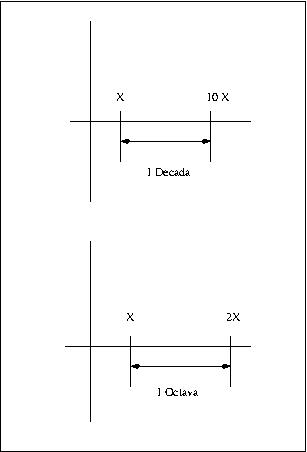
\includegraphics[height=6in, width=4in]{./graphics/decoct.png}
	\caption{D\'{e}cadas y octavas}
	\label{decoctpng}
\end{figure}


\subsubsection{Propiedades de las escalas en dB}

En todas las clases de dB, un factor de $10$ en la amplitud de la
se\~{n}al medida corresponde a un incremento de $20$ decibeles
\begin{equation}
  20 \, log_{10}(\frac{10 |A_{m}|}{|A_{r}|}) = 20 \, log_{10}(10) + 20 \, log_{10}(\frac{|A_{m}|}{|A_{r}|}).
\end{equation}

Una funci\'{o}n $f(x)$ que es proporcional a $\frac{1}{x}$ se dice que
``cae'' o disminuye a una raz\'{o}n de $20 dB$ por d\'{e}cada. Esto es, por cada
factor de $10$ en $x$ (cada d\'{e}cada), la amplitud cae $20 dB$.

En forma similar, un factor de $2$ en la amplitud corresponde a una
variaci\'{o}n de (aproximadamente) $6 dB$:
\begin{equation}
  20 \, log_{10} (\frac{2 |A_{m}|}{|A_{r}|}) = 20 \, log_{10}(2) + 20 \, log_{10}(\frac{|A_{m}|}{|A_{r}|}).
\end{equation}
Una funci\'{o}n que es proporcional a $\frac{1}{x}$ se dice que cae $6
dB$ por octava, o sea que por cada factor de $2$ en $x$ (por cada
octava) la amplitud disminuye aproximadamente $6 dB$. Entonces $6 dB$
por octava equivale a $20 dB$ por d\'{e}cada.

Finalmente, observemos que la elecci\'{o}n de la referencia determina
el desplazamiento vertical en la escala de $dB$:
\begin{equation}
  20 \, log_{10}(\frac{|A_{m}|}{|A_{r}|}) = 20 \, log_{10} (|A_{m}|) - 20 \, log_{10} (|A_{r}|),
\end{equation}
donde $-20 \, log_{10} (|A_{r}|)$ es el desplazamiento constante de la
escala vertical.

\subsubsection{Escalas en dB}

Dado que frecuentemente cambiamos las escalas de nuestras se\~{n}ales
para acomodarlas a nuestras necesidades parece ser in\'{u}til en
preocuparse por cu\'{a}l es la referencia de la escala en $dB$.  Sin
embargo, hay algunas escalas que debemos conocer.

\paragraph{Escala dBm} 
La referencia de potencia es $1 mW$ disipado en un
resistor de $600 \Omega$.

\paragraph{Escala dBV} 
La referencia de amplitud es $1$ volt. Entonces una se\~{n}al de $100$
volts equivale a
\begin{equation}
  20 log_{10} (\frac{100}{1}) = 40 dBV.
\end{equation}

\paragraph{Escala dB SPL} 
La referencia es la amplitud de una sinusoide de $1000$ hz de
frecuencia que ejerce una presi\'{o}n de $20 \, mBar = 20 \, \mu Pa$.
En unidades de intensidad sonora la referencia es igual a
\begin{equation}
  I_{0} = 10^{-16} \frac{W}{cm^{2}}.
\end{equation}
Dado que el sonido se crea mediante una presi\'{o}n variante en el
tiempo, calculamos niveles de sonido en $dB \, SPL$ usando la intensidad
promedio (calculada a lo largo de por lo menos un per\'{\i}odo de la
menor frecuencia contenida en el sonido).

\begin{tabular}{ll}
  Sonido                                          &       dB SPL  \\
  Motor jet a tres metros                         &       140     \\
  Umbral de dolor                                 &       130     \\
  Concierto de Rock                               &       120     \\
  Moto acelerando a cinco metros                  &       110     \\
  Martillo neum\'{a}tico a dos metros             &       100     \\
  F\'{a}brica                                     &       90      \\
  Aspiradora                                      &       80      \\
  Tr\'{a}fico pesado                              &       70      \\
  Restaurante quieto                              &       50      \\
  Area residencial a la noche                     &       40      \\
  Cine vacio                                      &       30      \\
  Murmullo de hojas secas                         &       20      \\
  Respiraci\'{o}n de una persona a tres metros    &       10      \\
  Umbral de audici\'{o}n                          &       0       
\end{tabular}

\paragraph{Escala dB para gr\'{a}ficos} 
La referencia elegida es la m\'{a}xima amplitud de la se\~{n}al:  Normalizamos la se\~{n}al tomando la m\'{a}xima amplitud como referencia,
a la que le corresponderá una medida en decibeles de $0 dB$. 
Para poder realizar esta normalizaci\'{o}n es evidente que necesitamos
conocer la se\~{n}al en un lapso de tiempo. Despu\'{e}s de encontrar
el m\'{a}ximo en dicho intervalo reci\'{e}n podemos realizar los
c\'{a}lculos.

\subsection{Ejemplo: Energ\'{\i}a promedio para la exponencial imaginaria de tiempo continuo en un período $T_{0}$}

Calculemos la energ\'{\i}a promedio de la exponencial imaginaria
en su per\'{\i}odo
\begin{equation}
  E_{T_{0}}=\int_{0}^{T_{0}}\left| e^{j \, \omega_{0} \, t}\right|
  ^{2}dt=\int_{0}^{T_{0}}\left( \cos \left( \omega_{0} \, t\right) ^{2}+\sin
    \left( \omega_{0} \, t\right) ^{2}\right) dt=T_{0}. \label{potfmuno}
\end{equation}

\subsection{Ejemplo: Potencia promedio para la exponencial imaginaria de tiempo continuo en un período $T_{0}$}

Calculemos su potencia promedio en un per\'{\i}odo $T_{0}$ 
\begin{equation}
  P_{T_{0}}=\frac{1}{T_{0}}E_{T_{0}}=\frac{1}{T_{0}}T_{0}=1. \label{potfmdos}
\end{equation}

\subsection{Ejemplo: Potencia promedio para la exponencial imaginaria de tiempo continuo en lapso de tiempo infinito}

Calculemos ahora su potencia promedio
\begin{equation}
  P_{\infty }= 
  \begin{array}{l}
    Lim \\ 
    T_{0}\rightarrow \infty
  \end{array}
  \frac{1}{2T_{0}}\int_{-T_{0}}^{T_{0}}\left| e^{j \, \omega_{0} \, t}\right|^{2}dt.
\end{equation}
\begin{equation}
  P_{\infty }= 
  \begin{array}{l}
    Lim \\ 
    T_{0}\rightarrow \infty
  \end{array}
  \frac{2T_{0}}{2T_{0}}=1.
\end{equation}

\subsection{Ejemplo: Energ\'{\i}a y potencia para señales de tiempo discreto}

\begin{enumerate}

\item Calculemos los valores de $E_{\infty }$ y $P_{\infty }$ para 
el escal\'{o}n $x_{1}\left[ n\right] =u[n]$.
Planteamos la f\'{o}rmula de energ\'{\i}a
  \begin{equation}
    E_{\infty }\left( x_{1}\left[ n\right] \right) = 
    \begin{array}{c}
      Lim \\ 
      N\rightarrow \infty
    \end{array}
    \sum_{n=-N}^{N}\left( u\left[ n\right] \right) ^{2},
  \end{equation}
Considerando que el escal\'{o}n es nulo ($u[n] = 0$) para $n$ negativo
$n < 0$, cambiamos el l\'{\i}mite inferior de la sumatoria a $0$. Dado
que el escal\'{o}n es igual a $1$ para $n$ no negativo ($n \geq 0$), reemplazamos $u(n)$
por $1$. Entonces resolvemos 
  \begin{equation}
    E_{\infty }\left( x_{1}\left[ n\right] \right) = 
    \begin{array}{c}
      Lim \\ 
      N\rightarrow \infty
    \end{array}
    \sum_{n=0}^{N} 1 =\infty.
  \end{equation}
Planteamos la f\'{o}rmula de potencia
  \begin{equation}
    P_{\infty }\left( x_{1}\left[ n\right] \right) = 
    \begin{array}{c}
      Lim \\ 
      N\rightarrow \infty
    \end{array}
    \frac{\sum_{n=-N}^{N}\left( u\left[ n\right] \right) ^{2}}{2N+1},
  \end{equation}
y con las mismas consideraciones que para el c\'{a}lculo de la
energ\'{i}a resolvemos
  \begin{equation}
    P_{\infty }\left( x_{1}\left[ n\right] \right) = 
    \begin{array}{c}
      Lim \\ 
      N\rightarrow \infty
    \end{array}
    \frac{\sum_{n=0}^{N}1}{2N+1}=\frac{1}{2}.
  \end{equation}

\item Calculemos los valores de $E_{\infty }$ y $P_{\infty }$ para 
$x_{2}[n]=2^{-n}u\left[ n\right].$
Planteamos la f\'{o}rmula de energ\'{\i}a
  \begin{equation}
    E_{\infty }\left( x_{2}\left[ n\right] \right) = 
    \begin{array}{c}
      Lim \\ 
      N\rightarrow \infty
    \end{array}
    \sum_{n=-N}^{N}\left( 2^{-n}u\left[ n\right] \right) ^{2}.
  \end{equation}
Considerando que el escal\'{o}n es nulo ($u[n] = 0$) para $n$ negativo
($n < 0$), cambiamos el l\'{\i}mite inferior a $n = 0$. Dado que el escal\'{o}n
es igual a $1$ ($u[n] = 1$) para $n$ no negativo ($n \geq 0$), reemplazamos $u[n]$ por $1$.
Resolvemos
  \begin{equation}
    E_{\infty }\left( x_{2}\left[ n\right] \right)= 
    \begin{array}{c}
      Lim \\ 
      N\rightarrow \infty
    \end{array}
    \sum_{n=0}^{N}\left( 4^{-n}\right) =\frac{1}{1-\frac{1}{4}}=\frac{4}{3},
  \end{equation}
aplicando la propiedad de las sumas geom\'{e}tricas
\begin{equation}
  \sum_{n = 0}^{N} q^{n} = \frac{1-q^{N+1}}{1-q},
\end{equation}
y su l\'{\i}mite
\begin{equation}
  \begin{array}{c}
    Lim \\
    n \rightarrow \infty
  \end{array}
  \frac{1-q^{n+1}}{1-q} =   \frac{1}{1-q},
\end{equation}
para $\parallel q \parallel_{2} < 1$.
Planteamos la f\'{o}rmula de potencia
  \begin{equation}
    P_{\infty }\left( x_{2}\left[ n\right] \right) = 
    \begin{array}{c}
      Lim \\ 
      N\rightarrow \infty
    \end{array}
    \frac{\sum_{n=-N}^{N}\left( 2^{-n}u\left[ n\right] \right) ^{2}}{2N+1},
  \end{equation}
y con las mismas consideraciones que para el c\'{a}lculo de la
energ\'{i}a resolvemos
  \begin{equation}
    P_{\infty }\left( x_{2}\left[ n\right] \right) = 
    \begin{array}{c}
      Lim \\ 
      N\rightarrow \infty
    \end{array}
    \frac{\frac{4}{3}}{2N+1}=0.
  \end{equation}

\item Calculamos los valores de $E_{\infty }$ y $P_{\infty }$ para 
$x_{3}\left[ n\right] =u\left[ n\right] -u\left[ n-2\right]$.
Planteamos la f\'{o}rmula de energ\'{\i}a
\begin{equation}
E_{\infty }\left( x_{3}\left[ n\right] \right) = 
\begin{array}{c}
Lim \\ 
N\rightarrow \infty
\end{array}
\sum_{n=-N}^{N}\left( u\left[ n\right] -u\left[ n-2\right] \right) ^{2}.
\end{equation}
Observemos que la funci\'{o}n es igual a $1$ para $0 \leq n < 2$, e
igual a $0$ para $n < 0$ y $n \leq 2$.Por lo tanto los l\'{\i}mites
de la sumatoria pueden cambiarse a $n = 0$ y $n = 2$.
Podemos resolver
\begin{equation}
E_{\infty }\left( x_{3}\left[ n\right] \right) = 
\begin{array}{c}
Lim \\ 
N\rightarrow \infty
\end{array}
2=2.
\end{equation}
Planteamos la f\'{o}rmula de potencia
\begin{equation}
P_{\infty }\left( x_{3}\left[ n\right] \right) = 
\begin{array}{c}
Lim \\ 
N\rightarrow \infty
\end{array}
\frac{\sum_{n=-N}^{N}\left( u\left[ n\right] -u\left[ n-2\right] \right)
^{2}}{2N+1},
\end{equation}
y resolvemos
\begin{equation}
P_{\infty }\left( x_{3}\left[ n\right] \right) = 
\begin{array}{c}
Lim \\ 
N\rightarrow \infty
\end{array}
\frac{2}{2N+1}=0.
\end{equation}

\item Calculamos los valores de $E_{\infty }$ y $P_{\infty }$ para 
$x_{4}\left[ n\right] =
  \cos \left( \frac{\pi }{4}n\right) \left( u\left[ n\right] -u\left[
      n-4\right] \right)$.
Planteamos la f\'{o}rmula de energ\'{\i}a
\begin{equation}
E_{\infty }\left( x_{4}\left[ n\right] \right) = 
\begin{array}{c}
Lim \\ 
N\rightarrow \infty
\end{array}
\sum_{n=-N}^{N}\left( \cos \left( \frac{\pi }{4}n\right) \left( u\left[ n
\right] -u\left[ n-4\right] \right) \right) ^{2},
\end{equation}
y resolvemos
\begin{equation}
E_{\infty }\left( x_{4}\left[ n\right] \right) = 
\begin{array}{c}
Lim \\ 
N\rightarrow \infty
\end{array}
2=2,
\end{equation}
Planteamos la f\'{o}rmula de potencia
\begin{equation}
P_{\infty }\left( x_{4}\left[ n\right] \right) = 
\begin{array}{c}
Lim \\ 
N\rightarrow \infty
\end{array}
\frac{\sum_{n=-N}^{N}\left( \cos \left( \frac{\pi }{4}n\right) \left(
      u\left[ n\right] -u\left[ n-4\right] \right) \right)
  ^{2}}{2N+1}.
\end{equation}
y resolvemos
\begin{equation}
P_{\infty }\left( x_{4}\left[ n\right] \right) = 
\begin{array}{c}
Lim \\ 
N\rightarrow \infty
\end{array}
\frac{2}{2N+1}=0.
\end{equation}

\item Calculamos los valores de $E_{\infty }$ y $P_{\infty }$ para 
$x_{5}\left( t\right) =\cos \left( t\right)$.
Planteamos la f\'{o}rmula de energ\'{\i}a y resolvemos
\begin{equation}
E_{\infty }\left( x_{5}\left( t\right) \right) = 
\begin{array}{c}
Lim \\ 
T\rightarrow \infty
\end{array}
\int_{-T}^{T}\left( \cos \left( t\right) \right) ^{2}dt = \infty.
\end{equation}
Planteamos la f\'{o}rmula de potencia
\begin{equation}
P_{\infty }\left( x_{5}\left( t\right) \right) = 
\begin{array}{c}
Lim \\ 
T\rightarrow \infty
\end{array}
\frac{\int_{-T}^{T}\left( \cos \left( t\right) \right) ^{2}dt}{2T}= 
\begin{array}{c}
Lim \\ 
T\rightarrow \infty
\end{array}
\frac{T+\frac{1}{2}\sin \left( 2T\right) }{2T},
\end{equation}
y resolvemos
\begin{equation}
P_{\infty }\left( x_{5}\left( t\right) \right) = 
\begin{array}{c}
Lim \\ 
T\rightarrow \infty
\end{array}
\frac{T+\frac{1}{2}\sin \left( 2T\right) }{2T}=\frac{1}{2}.
\end{equation}

\item Calculamos los valores de $E_{\infty }$ y $P_{\infty }$ para 
$x_{6}\left( t\right) =e^{j\left( 2t+\frac{\pi }{4}\right) }$.
Planteamos la f\'{o}rmula de energ\'{\i}a
\begin{equation}
E_{\infty }\left( x_{6}\left( t\right) \right) = 
\begin{array}{c}
Lim \\ 
T\rightarrow \infty
\end{array}
\int_{-T}^{T}e^{-j\left( 2t+\frac{\pi }{4}\right) }e^{j\left( 2t+\frac{\pi }{%
4}\right) }dt.
\end{equation}
\begin{equation}
E_{\infty }\left(x_{6}\left( t\right) \right) = 
\begin{array}{c}
Lim \\ 
T\rightarrow \infty
\end{array}
2T=\infty ,
\end{equation}
Planteamos la f\'{o}rmula de potencia y resolvemos
\begin{equation}
P_{\infty }\left( x_{6}\left( t\right) \right) = 
\begin{array}{c}
Lim \\ 
T\rightarrow \infty
\end{array}
\frac{2T}{2T}=1.
\end{equation}
\end{enumerate}

\section{Transformaciones de la variable independiente}

\subsection{Definici\'{o}n}

Una se\~{n}al se puede transformar en otra manipulando su variable
independiente. Consideraremos transformaciones lineales con
coeficientes $a$ y $b$.

El coeficiente $b$ determina el desplazamiento en el tiempo: es decir,
si la se\~{n}al transformada est\'{a} adelantada o retrasada respecto
a la se\~{n}al original. Este coeficiente es denominado fase.

El coeficiente $a$ determina la rapidez en el tiempo: es decir, si la
se\~{n}al transformada est\'{a} ``comprimida'' o ``estirada'' respecto
a la se\~{n}al original.

\subsubsection{Tiempo continuo}
\begin{equation}
  f(t)\rightarrow f\left( at+b\right).
\end{equation}

\subsubsection{Tiempo discreto}
\begin{equation}
  f\left[ n\right] \rightarrow f\left[ an+b\right].
\end{equation}

\subsection{Ejemplos}

\begin{figure}
  \centering
  
\includegraphics[height=3in]{./py-graphics/target/contvart.png}
  \caption{Transformaci\'{o}n de la variable independiente (tiempo
    continuo)}
  \label{contvarteps}
\end{figure}

\begin{figure}
  \centering
  
\includegraphics[height=3in]{./py-graphics/target/discvart.png}
  \caption{Transformaci\'{o}n de la variable independiente (tiempo
    discreto)}
  \label{discvarteps}
\end{figure}

\begin{figure}
  \centering
  
\includegraphics[height=3in]{./py-graphics/target/contfase-1.png}
  \caption{Distintas fases (tiempo continuo)}
  \label{contfase.1}
\end{figure}

\begin{figure}
  \centering
  
\includegraphics[height=3in]{./py-graphics/target/contfase-2.png}
  \caption{Distintas fases (tiempo continuo)}
  \label{contfase.2}
\end{figure}

\begin{figure}
  \centering
  
\includegraphics[height=3in]{./py-graphics/target/contfrec.png}
  \caption{Distintas ``velocidades'' (tiempo continuo)}
  \label{contfreceps}
\end{figure}

\begin{figure}
  \centering
  
\includegraphics[height=3in]{./py-graphics/target/discfase.png}
  \caption{Distintas fases (tiempo discreto)}
  \label{discfaseeps}
\end{figure}

\begin{figure}
  \centering
  
\includegraphics[height=3in]{./py-graphics/target/discfrec.png}
  \caption{Distintas ``velocidades'' (tiempo discreto)}
  \label{discfreceps}
\end{figure}


\subsubsection{Transformaciones de la variable independiente, tiempo continuo}

\begin{enumerate}

\item Vea la Fig. (\ref{contvarteps}). Aqu\'{\i} se muestran
  variaciones de rapidez y fase en una se\~{n}al de tiempo continuo
  mediante las transformaciones de la variable tiempo $t$ indicadas
  sobre cada uno de los gr\'{a}ficos.

\item Vea la Fig. (\ref{contfase.1}).  Aqu\'{\i} se muestran
  variaciones de fase en una se\~{n}al de tiempo continuo.  Verifique
  el cambio de fase observando el valor de la se\~{n}al en
  cercan\'{\i}as de $t = 0$.

\item Vea la Fig. (\ref{contfase.2}). 

\item Vea la Fig. (\ref{contfreceps}). Aqu\'{\i} se muestran
  variaciones de velocidad en una se\~{n}al de tiempo continuo.
  Verifique el ``estiramiento'' o la ``compresi\'{o}n'' de la
  se\~{n}al contando los m\'{a}ximos.

\end{enumerate}


\subsubsection{Transformaciones de la variable independiente, tiempo discreto}

\begin{enumerate}

\item Vea la Fig. (\ref{discvarteps}).  Aqu\'{\i} se muestran
  variaciones de rapidez y fase en una se\~{n}al de tiempo discreto
  mediante las transformaciones de la variable tiempo $n$ indicadas
  sobre cada uno de los gr\'{a}ficos.

\item Vea la Fig. (\ref{discfaseeps}). Aqu\'{\i} se muestran
  variaciones de fase en una se\~{n}al de tiempo discreto.  Verifique
  el cambio de fase observando el valor de la se\~{n}al en
  cercan\'{\i}as de $n = 0$.

\item Vea la Fig. (\ref{discfreceps}). Aqu\'{\i} se muestran
  variaciones de velocidad en una se\~{n}al de tiempo discreto.
  Verifique el ``estiramiento'' o la ``compresi\'{o}n'' de la
  se\~{n}al contando los m\'{a}ximos.

\end{enumerate}


% \subsubsection{Aplicaci\'{o}n tecnol\'{o}gica}
% Una aplicaci\'{o}n tecnol\'{o}gica de la transformaci\'{o}n de
% variable independiente es la c\'{a}mara lenta del video.


%\section{Para practicar}
%
%\begin{enumerate}
%\item Elabore un breve resumen (con texto, f\'{o}rmulas y gr\'{a}ficos,
%  seg\'{u}n lo que sea posible) de los siguientes conceptos expuestos en esta
%  cap\'{i}tulo
%\begin{enumerate}
%\item Informaci\'{o}n, ruido, se\~{n}al, y sistema.
%\item Variable dependiente e independiente.
%\item Tiempo continuo y discreto.
%\item Se\~{n}ales finitas, e infinitas, causales y anticausales.
%\item Se\~{n}ales pares e impares.
%\item Se\~{n}ales peri\'{o}dicas.
%\item Energ\'{\i}a y potencia.
%\item Composici\'{o}n de se\~{n}ales.
%\end{enumerate}
%
%\item Identifique distintos criterios para identificar los distintos tipos de se\~{n}ales y sistemas que conozca.
%
%\item Busque en Internet sitios web de materias similares a esta, y
%  escriba un peque\~{n}o informe sobre ellos (no m\'{a}s de media p\'{a}gina).
%
%\item Busque en Internet la biograf\'{\i}a de Claude Shannon.
%  Escriba una descripci\'{o}n (en cinco a diez renglones) de la
%  obra de Claude Shannon y su impacto en la ingenier\'{\i}a
%  electr\'{o}nica.
%
%\item \textquestiondown Qu\'{e} se\~{n}ales aparecen en circuitos
%  el\'{e}ctricos y electr\'{o}nicos? 
%
%\item \textquestiondown Cu\'{a}l es la diferencia entre circuitos
%  el\'{e}ctricos y electr\'{o}nicos?
%
%\item \textquestiondown Como podemos hacer para trabajar con una
%  se\~{n}al no el\'{e}ctrica, como una temperatura, en un circuito
%  el\'{e}ctrico?
%
%\item Genere en matlab una se\~{n}al peri\'{o}dica de referencia
%  adecuada (elija frecuencia y amplitud).
%
%\item Genere en matlab una se\~{n}al cuya potencia sea un decibel
%  mayor que la se\~{n}al de referencia.
%
%\item Escuche por el parlante. Saque conclusiones.
%
%\item Genere en matlab se\~{n}ales cuya potencia sea 10 decibeles
%  inferior que la se\~{n}al de referencia, con frecuencias entre $50$
%  y $20000$ hz.
%
%\item Escuche por el parlante. Saque conclusiones.
%
%\item En el punto siguiente leeremos la descripci\'{o}n de una experiencia con
%  un circuito RC planteada en forma vaga e imprecisa. 
%  En grupos de dos a tres integrantes, escriban como 
%  deber\'{\i}a estar escrita la descripci\'{o}n en t\'{e}rminos de
%  interfaces de entrada y salida, y componentes.
%
%\item Dise\~{n}e un circuito con muchas resistencias y capacitores,
%  tal que conectando una fuente de alterna, se pueda medir el desfasaje
%  de los capacitores.
%
%\item En forma grupal, definamos una divisi\'{o}n de este circuito en
%  partes o componentes que cada uno de los integrantes pueda armar por
%  separado. \label{circuitorc}
%
%\item Escriba un programa matlab que repita (y mejore) gr\'{a}ficos de este cap\'{\i}tulo. 
%
%\item Grafique las siguientes se\~{n}ales y determine claramente cu\'{a}les
%son los intervalos de tiempo en los cuales estas son nulas o no nulas.
%\begin{enumerate}
%\item $x_{a}(t) = u(t) - u(1-t)$.
%\item $x_{b}(t) = u(t) \, u(1-t)$.
%\item $x_{c}(t) = u(t) \, u(1-t) + u(t+5) \, u(t+4)$.
%\item $x_{a}[n] = u[n] - u[n-2]$.
%\item $x_{b}[n] = u[n] \, u[n-2]$.
%\item $x_{c}[n] = \sum_{k=2}^{4} u[n-k] \, u[n-2 k]$.
%\end{enumerate}
%
%\item Consideremos las se\~{n}ales $x_{1}(t) = cos(2 \pi t)$ y
%  $x_{2}(t) = cos(4 \pi t)$.  \textquestiondown C\'{u}al de las dos
%  tiene m\'{a}s energ\'{\i}a en un lapso de tiempo $\Delta T = 1$?
%
%\item Consideremos las se\~{n}ales $cos(2 \pi t)$ y $cos(2 \pi t +
%  1)$. \textquestiondown C\'{u}al de las dos tiene m\'{a}s
%  energ\'{\i}a en un lapso de tiempo $\Delta T = 1$?
%
%\item Grabe los sonidos producidos por dos monedas diferentes al caer desde un escritorio.
%Explique como puede estimar las masas de ambas monedas operando sobre las grabaciones.
%
%\end{enumerate}

\section{Respuestas a algunas preguntas}

\begin{itemize}
\item \textquestiondown Cu\'{a}l es el valor de $p(1)$ que maximiza
  $H([0,1]) = p(1) \, log_{2} p(1) + (1 - p(1)) \, log_{2} (1 - p(1))$?
Dada $q(x) = x \, log_{2} x + (1 - x) \, log_{2} (1 - x)$, tenemos que obtener la ra\'{\i}z de 
$\frac{d q(x)}{d x} = 0$ o graficar $q(x)$ para $x \in [0, 1]$.
El resultado buscado es $p(1) = x = \frac{1}{2}$.

\item \textquestiondown C\'{u}al podr\'{i}a ser un ejemplo de reloj
  anal\'{o}gico de ``verdad''?  \textquestiondown Este reloj
  anal\'{o}gico de verdad ser\'{\i}a exacto ?
Los relojes de sol, los relojes de agua y arena, y las velas ardientes son relojes de tiempo continuo.
El problema intr\'{\i}nseco que tiene el manejo de la informaci\'{o}n ``continua'' es que no es reproducible con facilidad y se deteriora con rapidez ante la presencia inevitable de ruido.

\item \textquestiondown Qu\'{e} entiende por procesamiento, modelado y an\'{a}lisis de se\~{n}ales y sistemas?
\begin{itemize}
\item Procesamiento de se\~{n}ales: transformaci\'{o}n de una se\~{n}al en otra.

\item Modelado de se\~{n}ales y sistemas: usar un algoritmo y sus par\'{a}metros 
para reproducir o explicar caracter\'{\i}sticas de la se\~{n}al o sistemas en estudio, 
con el objetivo de realizar inferencias.

\item An\'{a}lisis de se\~{n}ales y sistemas: Obtenci\'{o}n de medidas.
\end{itemize}

\end{itemize}


